\documentclass[12pt,twoside,openright,a4paper]{report}
\usepackage{graphicx}
\DeclareGraphicsExtensions{.pdf, .png, .jpg}
\usepackage{tex_files/style}

\sloppy

\title{
    \textbf{{\Huge{Tropospheric Ozone Production \\Pathways with Detailed Chemical Mechanisms}}}\\ \vspace{2cm}
    \normalsize{{Dissertation zur Erlangung des akademischen Grades} \\
    {des Doktors der Naturwissenschaften} \\
    {am Fachbereich Geowissenschaften} \\
    {an der Freien Universit\"{a}t Berlin}\\} \vspace{2cm}
    \textbf{{Vorgelegt von} \\
    {Jane Coates} \\
    {im April 2016} \\} \vspace{3cm}
    {
\includegraphics[scale=0.5]{img/FU_logo}}
}
%removing author and date for maketitle
\author{\vspace{-5ex}}
\date{\vspace{-5ex}}

\begin{document}
\nobibliography*

\pagenumbering{Alph}
\maketitle
\clearpage{\pagestyle{empty}\cleardoublepage}

\thispagestyle{empty}
\newsavebox{\supervisors}
\sbox{\supervisors}{
    \begin{tabular}{ll}
        %\textbf{\large{1. Gutachter:}} & \textbf{\large{Dr. Tim Butler}} \\
        \textbf{\large{1. Gutachter:}} & \textbf{\large{Prof. Dr. Peter Builtjes}} \\
        \textbf{\large{2. Gutachter:}} & \textbf{\large{Prof. Dr. Martijn Schaap}} \\ [1cm]
        \textbf{\large{Tag der Disputation:}} & \textbf{\large{12.07.2016}}
    \end{tabular}
}
\begin{tikzpicture}
    \matrix [matrix of nodes] {
        \node (supervisors) [shift = {(2cm, -20cm)}, draw = none] at (current page.south west) {\usebox{\supervisors}}; \\
    };
\end{tikzpicture}
\clearpage{\pagestyle{empty}\cleardoublepage}

\clearpage{\pagestyle{empty}\cleardoublepage}

\pagenumbering{roman}

%\chapter*{Abstract}
%\clearpage{\pagestyle{empty}\cleardoublepage}
\chapter*{Acknowledgements}
First and foremost, I would like to thank Tim Butler. 
Thanks for giving me the opportunity to perform the work, bringing me up to speed on the skills I needed for the work and always being there to offer advice. 
Allowing a mathematician to step up to the world of atmospheric chemistry speaks very highly of you.
I also appreciate the criticism which helped me improve my work, your sense of humour and that we make a good basis for a successful pub quiz team!

Secondly, I would like to thank Mark Lawrence and the IASS Potsdam for scientific and financial support of the project.
Working at the IASS has not only helped to develop my disciplinary knowledge of atmospheric chemistry but also to keep in mind that scientific excellence alone is not the sole basis of societal transformation.
The interdisciplary and transdisciplinary approaches are needed to complement disciplinary work, I could not have truely understood this without working at the IASS Potsdam.

I thank Peter Builtjes for the collaboration and support during the project.
Your pleasant comments and input during the many PAC meetings is greatly appreciated.

Thanks also goes to all my colleagues, past and present, at the IASS Potsdam.
All the discussions, translating, running breaks, cake breaks and coffee breaks helped me throughout this time!

Last but not least, I must thank Nadja Menz: you have sat through so many trial presentations, proofread texts and supplied an adequate amount of coffee and baked goodies to fuel me through this work. 
For your unwaivering support that takes on many forms - thanks!

\clearpage{\pagestyle{empty}\cleardoublepage}

\singlespacing
\tableofcontents{\fancyhead[LE]{\contentsname}\fancyhead[RE]{}}
\onehalfspacing
\clearpage{\pagestyle{empty}\cleardoublepage}
\listoftables{\fancyhead[LE]{\contentsname}\fancyhead[RE]{}}
\clearpage{\pagestyle{empty}\cleardoublepage}
\listoffigures{\fancyhead[LE]{\contentsname}\fancyhead[RE]{}}
\clearpage{\pagestyle{empty}\cleardoublepage}

\fancyhf{}
\fancyhead[RO,LE]{Tropospheric Ozone Production Pathways}
\fancyhead[LO,RE]{Chapter \thechapter}
\fancyfoot{}
\fancyfoot[LE,RO]{\thepage}
\fancyfoot[LO,RE]{Jane Coates}
\renewcommand{\headrulewidth}{2pt}
\renewcommand{\footrulewidth}{1pt}
\chapter{Introduction} \label{c:introduction}
\pagenumbering{arabic}
Air pollution is the leading environmental health risk in many areas around the world.
The effects of air pollution to the general population range from chronic to less severe health impacts and reduced growth rates of vegetation resulting in economic losses of billions of euros \citep{AQEU:2015}.
Moreover, the International Agency for Research on Cancer labelled air pollution as carcinogenic \citep{IARC:2013}.
Due to these impacts, many governed areas introduced legislation designed to reduce concentrations of many air pollutants.

Tropospheric ozone (\ce{O3}) is one of the most problematic air pollutants over Europe with up to $98$~\% of Europe's urban population exposed to concentrations of ozone above the WHO guidelines \citep{AQEU:2015}.
Furthermore, in 2011 the EU ozone target value for human health (the EU has no limit value for ozone) was exceeded in $65$~\% of the EU member states and Europe's ozone target value for vegetation was exceeded in $27$~\% of the EU-28 agricultural areas \citep{AQEU:2013}.

Reducing atmospheric concentrations of tropospheric ozone is a complex problem as ozone is not directly emitted into the troposphere.
Tropospheric ozone is produced from the reactions of volatile organic compounds (VOCs) in the presence of nitrogen oxides \mbox{(\ce{NO_x}~$\equiv$~NO + \ce{NO2})} and sunlight \citep{Atkinson:2000}.
Meteorology and transport also influence tropospheric ozone levels \citep{Jacob:2009}.

Air quality (AQ) models are an important tool for understanding ozone pollution and predicting future air quality.
Many AQ models are available with different scales and dimensions depending on the scope of the modelling experiment.
Accurately representing the complexity of ozone production in a computationally efficient model is an ongoing challenge for the modelling community \citep{Russell:2000}.

Model intercomparison projects (MIPs) compare the outputs from different models showing differences in tropospheric ozone due to differing representations of key processes.
For example, ACCMIP (Atmospheric Chemistry and Climate Model Intercomparison Project) showed different magnitudes of future ozone burden in the same region \citep{Young:2013}.
A current MIP, CCMI (Chemistry Climate Model Initiative), aims to investigate differences in the representation of chemistry, emissions and transport processes between models to understand the differences between predictions from global models \citep{Eyring:2013}.

Detailed process studies are key to understanding differences between simulated ozone levels from different models.
This thesis determines the effects of VOC degradation chemistry, VOC emissions and temperature on modelled ozone predictions.
This assessment should be beneficial to the modelling community in understanding potential differences between model outputs and improving AQ models.

\section{Ozone} \label{s:ozone}
%atmospheric O3 with budget, lifetime, stratospheric & tropospheric ozone
Ozone is a atmospheric gas found in the stratosphere and troposphere, however its atmospheric effects are very different in these regions.
The stratosphere contains $\sim$~90~\% of the atmospheric ozone with a peak mixing ratio of $\sim$~$12$~ppm \citep{Seinfeld:2006}.
Stratospheric ozone absorbs the sun's ultraviolet radiation which is important due to the adverse effects of excess UV radiation on humans and ecosystems.

In contrast, tropospheric (or surface) ozone is both a pollutant and a greenhouse gas. 
Increased levels of tropospheric ozone are harmful to humans, plants and other living systems. 
High ozone exposure may lead to pulmonary problems in humans and can decrease both crop yields and forest growth \citep{WMO:2010}. 

Tropospheric ozone is formed via photochemical production from the reactions between VOCs and \ce{NO_x}, described in Sect.~\ref{s:ozone_chemistry}, while meteorology and atmospheric transport also influence ozone concentrations.
For example, a spring-time peak in tropospheric ozone is common in the Northern Hemisphere (NH) mid-latitudes, originally attributed to transport of ozone from the stratosphere into the troposphere via the Stratosphere-Troposphere Exchange (STE) \citep{Monks:2000}.
However, ozone transported via the STE rarely influences surface ozone levels \citep{Lelieveld:2000} and the spring maximum is due to the photochemical reactions occuring in the NH spring after the buildup of reservoir species over winter \citep{Penkett:1986}.
%These reservoir species are oxidised at a faster rate due to the spring-time increase in temperature, moisture and sunlight.

Understanding the intracacies of surface ozone pollution requires a combined effort from the modelling, observational and chemical kinetic communities -- called the ``three-legged stool'' approach by \citet{Abbatt:2014}.
Modelling of ozone production helped understand the complexity of atmospheric chemistry, such as the non-linear relationship of ozone production with precursor (VOC and \ce{NO_x}) emissions.
Modelling studies attempt to reproduce observational trends of surface ozone and model predictions may inspire new observational studies.
Chemical kinetic studies performed by laboratories give insights to missing or incorrect representations of atmospheric chemistry to be included in updated models.

This thesis focuses on the influence on ozone production from the representation of VOC degradation chemistry, VOC emissions and the ozone-temperature relationship within models.
Ozone production chemistry is outlined in Sect.~\ref{s:ozone_chemistry}, while sources of emissions of ozone precursors are described in Sect.~\ref{s:precursor_emissions}.
Finally, the effects of meteorology, in particular temperature, on ozone production are presented in Sect.~\ref{s:meteo_ozone}.
For the rest of this thesis, ozone refers to tropospheric ozone.

\section{Ozone Chemistry} \label{s:ozone_chemistry}
Ozone absorbs UV radiation producing either ground-state atomic oxygen (\ce{O(^3P)}) or excited singlet (\ce{O(^1D)}) oxygen atoms.
\begin{rxnarray}
    \ce{O3 + h\nu} & \rightarrow \ce{O2 + O(^3P)} \label{r:O3_hva} \\
    \ce{O3 + h\nu} & \rightarrow \ce{O2 + O(^1D)} \label{r:O3_hvb} 
\end{rxnarray}
Ground-state oxygen quickly reacts with oxygen to reform ozone.
\begin{rxnarray}
    \ce{O(^3P) + O2} & \xrightarrow[]{\text{\tiny{M}}} \ce{O3} \label{r:O_O2}
\end{rxnarray}
Thus there is no net loss or production of ozone through \eqref{r:O3_hva} and \eqref{r:O_O2}.
\ce{O(^1D)} may collide with \ce{N2} or \ce{O2} (represented as M in chemical reactions) stabilising to the ground-state.
%\begin{rxnarray}
    %\ce{O(^1D)} & \xrightarrow[]{\text{\tiny{M}}} \ce{O(^3P)} \label{r:O1D_M} 
%\end{rxnarray}
This process again leads to a null cycle with ozone destruction balanced by production.
However, \ce{O(^1D)} can react with water vapour producing hydroxyl (OH) radicals.
The OH radical is a highly reactive chemical species reacting with almost all trace chemical species in the troposphere.
\citep{Seinfeld:2006, Monks:2005}
\begin{rxnarray}
    \ce{O(^1D) + H2O} & \rightarrow \ce{2 OH} \label{r:O1D_H2O}
\end{rxnarray} 

The initial oxidation of VOCs by OH initiates a reaction chain which may lead to net production or loss of ozone depending on the atmospheric conditions.
For example, when carbon monoxide (CO) reacts with OH in the presence of oxygen, carbon dioxide and the hydroperoxy (\ce{HO2}) radical are formed.
In polluted areas with high-\ce{NO_x} concentrations, \ce{HO2} readily reacts with nitrogen oxide (NO) regenerating OH and producing nitrogen dioxide (\ce{NO2}).
\begin{rxnarray}
    \ce{CO + OH} & \xrightarrow[]{\ce{O2}} \ce{HO2 + CO2} \label{r:CO_OH} \\
    \ce{HO2 + NO} & \rightarrow \ce{OH + NO2} \label{r:HO2_NO}
\end{rxnarray}
Photolysis of \ce{NO2} produces ground-state atomic oxygen leading to ozone production via \eqref{r:O_O2}.  
\begin{rxnarray}
    \ce{NO2 + h\nu} & \rightarrow \ce{NO + O(^3P)} \label{r:NO2_hv} 
\end{rxnarray}
%OH may also react with NO to produce nitrous oxide (HONO), which rapidly photolyses to return OH and NO.
%\begin{rxnarray}
    %\ce{OH + NO} & \rightarrow \ce{HONO} \label{r:OH_NO} \\
    %\ce{HONO + h\nu} & \rightarrow \ce{OH + NO} \label{r:HONO_hv}
%\end{rxnarray}
The reaction between OH and \ce{NO2} produces nitric acid (\ce{HNO3}) limiting the recycling of OH and \ce{NO2}.
Nitric acid may be removed through deposition processes and is a sink for both OH and \ce{NO2}.
\begin{rxnarray}
    \ce{NO2 + OH} \rightarrow \ce{HNO3} \label{r:NO2_OH}
\end{rxnarray}

In low-\ce{NO_x} conditions away from polluted areas, OH and \ce{HO2} are interconverted through reactions with ozone.
\begin{rxnarray}
    \ce{OH + O3} & \rightarrow \ce{HO2 + O2} \label{r:OH_O3} \\
    \ce{HO2 + O3} & \rightarrow \ce{OH + 2 O2} \label{r:HO2_O3}
\end{rxnarray}
OH and \ce{HO2} may also react in a termination reaction producing water vapour and oxygen.
\begin{rxnarray}
    \ce{HO2 + OH} \rightarrow \ce{H2O + O2} \label{r:HO2_OH}
\end{rxnarray}
Other termination reactions involve combination reactions of \ce{HO2} radicals producing hydrogen peroxide (\ce{H2O2}).
\begin{rxnarray}
    \ce{HO2 + HO2} & \rightarrow \ce{H2O2} \label{r:HO2_HO2}
\end{rxnarray}
Hydrogen peroxide may be removed through deposition \citep{Gunz:1990} but may also be a temporary sink for the odd-oxygen species OH and \ce{HO2}.
\begin{rxnarray}
    \ce{H2O2 + h\nu} & \rightarrow \ce{2 OH} \label{r:H2O2_hv} \\
    \ce{H2O2 + OH} & \rightarrow \ce{HO2 + H2O} \label{r:H2O2_OH}
\end{rxnarray}
In summary, the secondary degradation of CO produces ozone in high-\ce{NO_x} conditions while in low-\ce{NO_x} conditions ozone is destroyed.
\citep{Seinfeld:2006, Monks:2005}

\begin{figure}[t]%
    \begin{center}%
        \caption[Methane degradation pathways]{Methane degradation pathways in low-\ce{NO_x} and high-\ce{NO_x} conditions. Taken from \citet{Monks:2005}.}%
        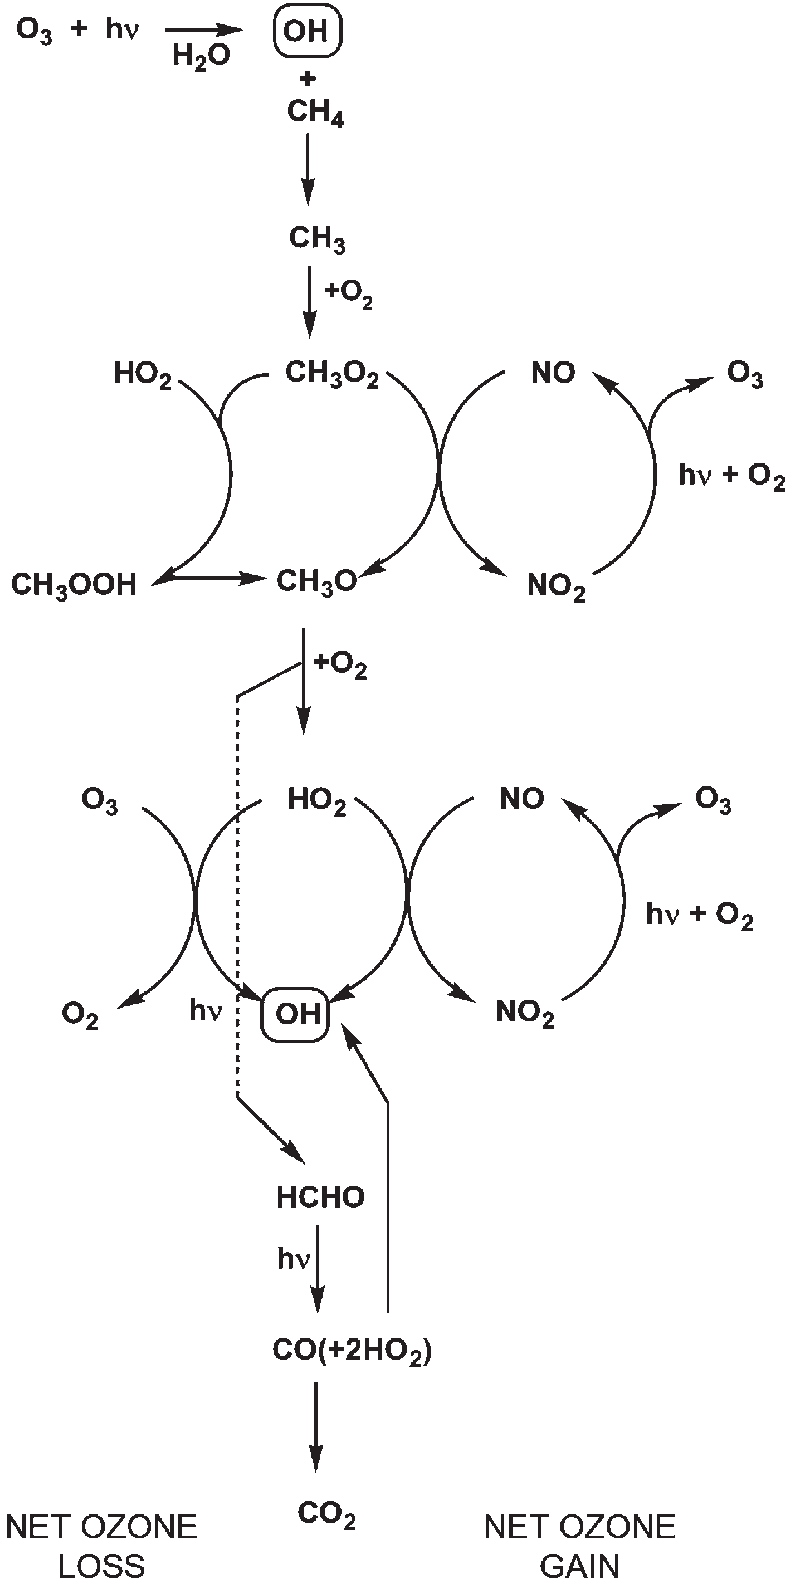
\includegraphics[scale = 0.45]{CH4_degradation}%
        \label{f:CH4_oxidation}%
    \end{center}%
\end{figure}%
The secondary degradation of more complex VOCs has similar features to that of CO.
Methane (\ce{CH4}), with a mixing ratio of $\sim$~$1.7$~ppmv, is the most abundant VOC in the troposphere.
The reaction of methane with OH, in the presence of \ce{O2}, produces the methyl peroxy radical (\ce{CH3O2}) -- the simplest organic peroxy radical (\ce{RO2}).
\begin{rxnarray}
    \ce{CH4 + OH} \xrightarrow[]{\ce{O2}} \ce{CH3O2 + H2O} \label{r:CH4_OH}
\end{rxnarray}
Similar to CO oxidation, \ce{NO_x} conditions play a crucial role in the fate of \ce{CH3O2} and whether ozone is produced or destroyed, depicted in Fig.~\ref{f:CH4_oxidation}.

\begin{figure}[t]%
    \begin{center}%
        \caption[Schematic of general secondary degradation of VOCs]{Schematic diagram outlining general pathways of the secondary degradation of an emitted VOC.}%
        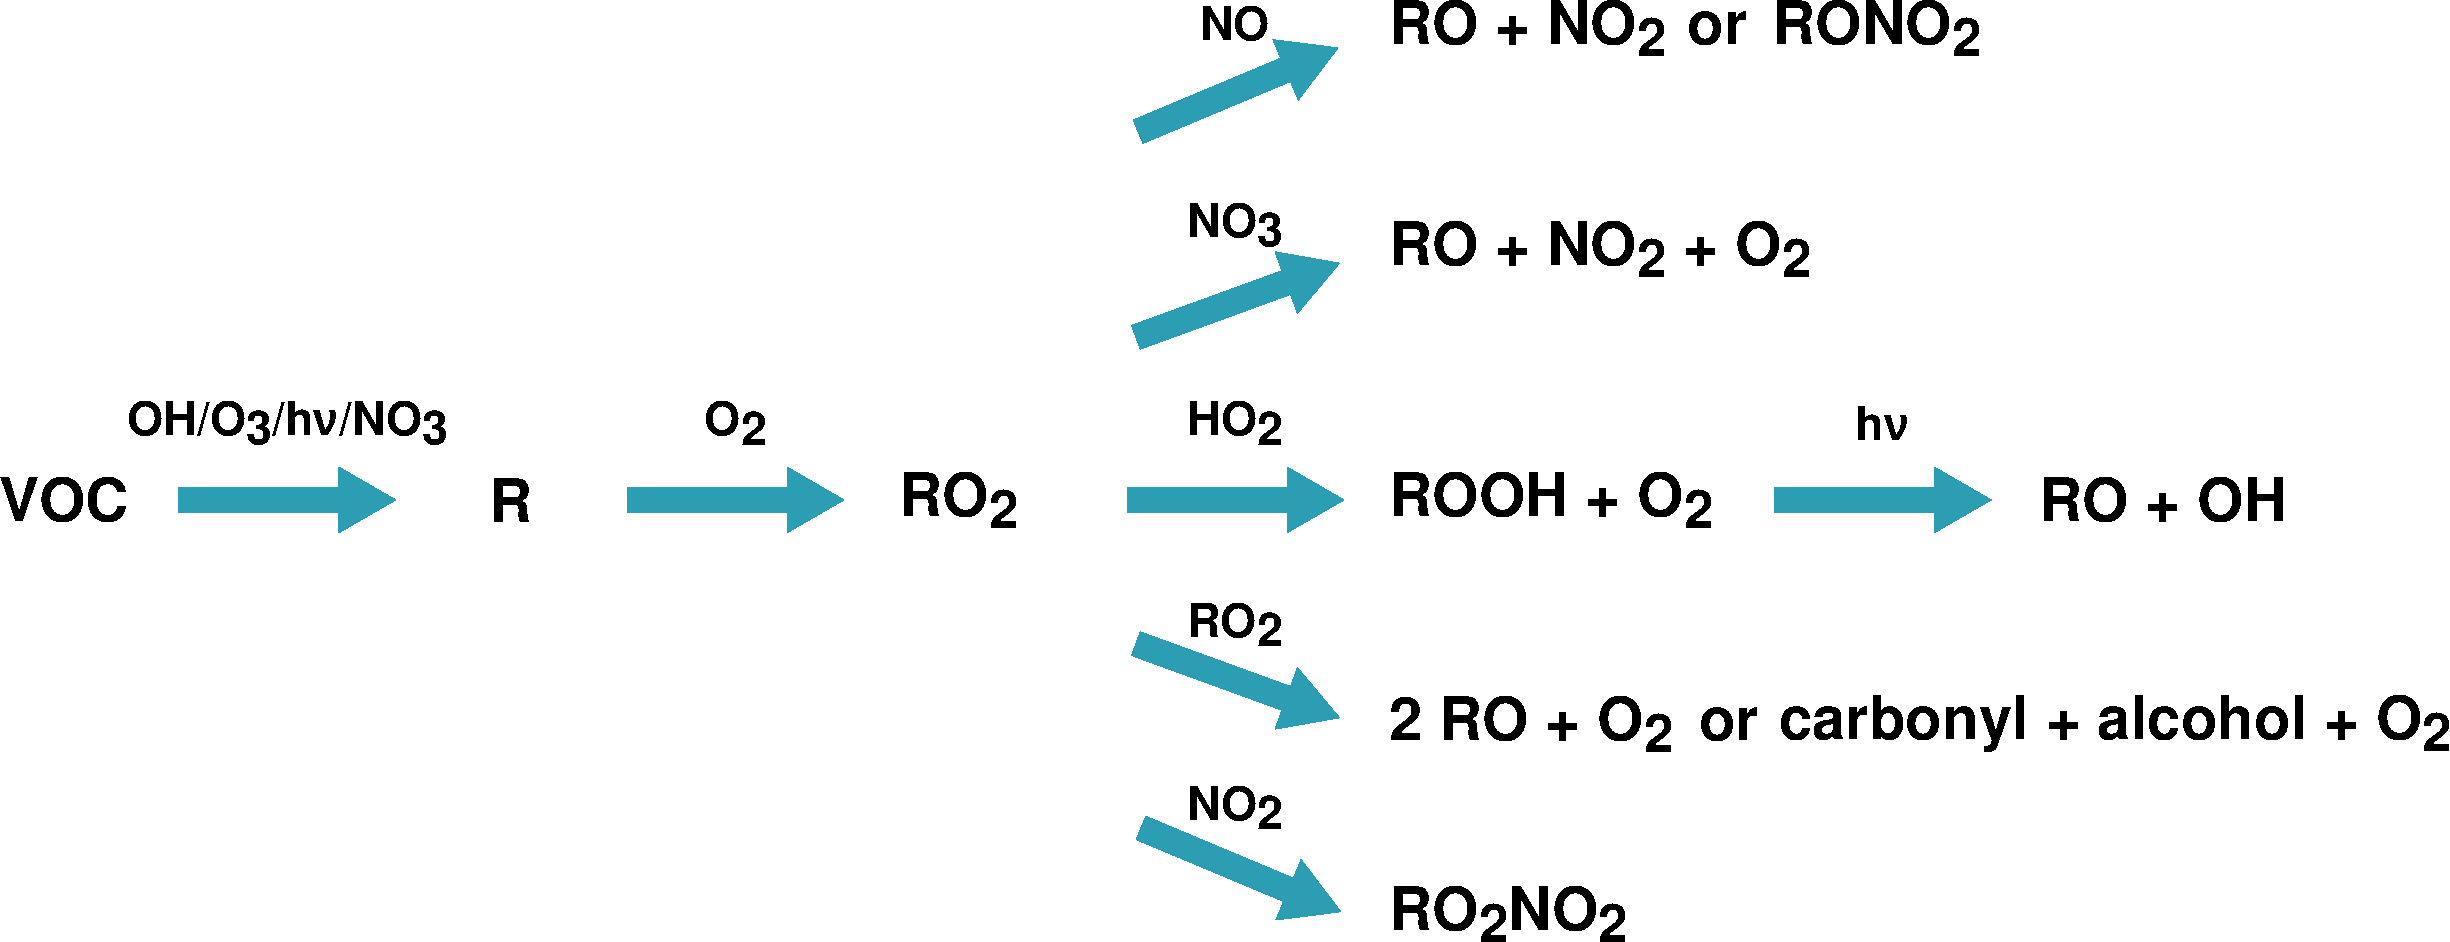
\includegraphics[width = \textwidth]{VOC_degradation}%
        \label{f:VOC_reaction}%
    \end{center}%
\end{figure}%
The general types of secondary degradation products formed during \ce{CH4} degradation can be extended to more complex non-methane VOCs (NMVOCs).
Initial oxidation pathways of NMVOCs are reaction with OH, while unsaturated VOCs, such as alkenes, may react with ozone and photolysis is important for carbonyl species.
During the night-time, reaction with the nitrate (\ce{NO3}) radical is typically more important than OH-oxidation due to the relatively higher concentrations of \ce{NO3} during night-time.  
\begin{rxnarray}
    \ce{VOC + OH / NO3 / O3 / h\nu} & \xrightarrow[]{\ce{O2}} \ce{RO2} \label{r:VOC_init} 
\end{rxnarray} 

Figure~\ref{f:VOC_reaction} represents a general and simplified reaction scheme for VOCs in the troposphere. 
The initial oxidation of NMVOC produces \ce{RO2} radicals and the fate of the \ce{RO2} determines whether net loss or production of ozone occurs.
\begin{rxnarray}
    \ce{RO2 + NO} & \xrightarrow[]{\text{M}} \ce{RONO2} \label{r:RO2_NOa} \\
    \ce{RO2 + NO} & \rightarrow \ce{RO + NO2} \label{r:RO2_NOb} \\
    \ce{RO2 + NO2} & \xrightleftharpoons[]{\text{M}} \ce{RO2NO2} \label{r:RO2_NO2} \\
    \ce{RO2 + NO3} & \rightarrow \ce{RO + NO2 + O2} \label{r:RO2_NO3} \\
    \ce{RO2 + HO2} & \rightarrow \ce{ROOH + O2} \label{r:RO2_HO2} \\
    \ce{RO2 + RO2} & \rightarrow \ce{2RO + O2} \label{r:RO2_RO2a} \\
    \ce{RO2 + RO2} & \rightarrow \ce{RCH(OH)R + RC(O)R + O2} \label{r:RO2_RO2b}
\end{rxnarray}
All degradation pathways of \ce{RO2} that produce \ce{NO2} result in \ce{O3} formation due to \eqref{r:NO2_hv} and \eqref{r:O_O2}. 
Reaction with the \ce{HO2} radical forms a hydroperoxide (ROOH) which may either be removed from the system or photolysed producing an alkoxy (RO) radical and OH.
The carbonyl and alcohol products resulting from reactions between \ce{RO2} radicals follows a similar sequence of reactions and can produce further \ce{O3}. 
Thus the subsequent reactions of secondary degradation products of a VOC may lead to further production of ozone.

Reaction of \ce{RO2} with \ce{NO2} \eqref{r:RO2_NO2} forms peroxy nitrates (\ce{RO2NO2}) which are a temporary reservoir for \ce{RO2} and \ce{NO_x}.
The thermal decomposition rate of \ce{RO2NO2} is highly temperature dependent.
At lower temperatures, \ce{RO2NO2} builds up and may be transported away from the region of formation. 
Thus releasing \ce{RO2} and \ce{NO2} in areas away from large sources of \ce{NO_x} and fuelling ozone production.
%This is one example of the dependence of ozone production on meteorological variables, a broader overview is given in Sect.~\ref{s:meteo_ozone}.

The reaction between NO and ozone is another important reaction in polluted regions.
\begin{rxnarray}
    \ce{NO + O3} & \rightarrow \ce{NO2 + O2} \label{r:NO_O3}
\end{rxnarray}
Reactions \eqref{r:NO_O3}, \eqref{r:NO2_hv} and \eqref{r:O_O2} form a null cycle of ozone production and destruction which limits ozone levels.
On the local urban scale close to NO sources, \eqref{r:NO_O3} decreases ozone levels called ozone titration.
Ozone titration is also important during the night where the lack of photochemistry does not regenerate ozone.
Urban measurement studies have confirmed the importance of ozone titration near source of NO \citep{Syri:2001}.

\subsection[VOC and NOx Chemistry]{VOC and \ce{NO_x} Chemistry} \label{ss:VOC_NOx}
\begin{figure}%
	\begin{center}%
        \caption[Ozone mixing ratios as a function of \ce{NO_x} and VOCs]{Ozone isopleth plots for various initial mixing ratios of \ce{NO_x} and VOCs. Taken from \citet{Jenkin:2000}.}%
        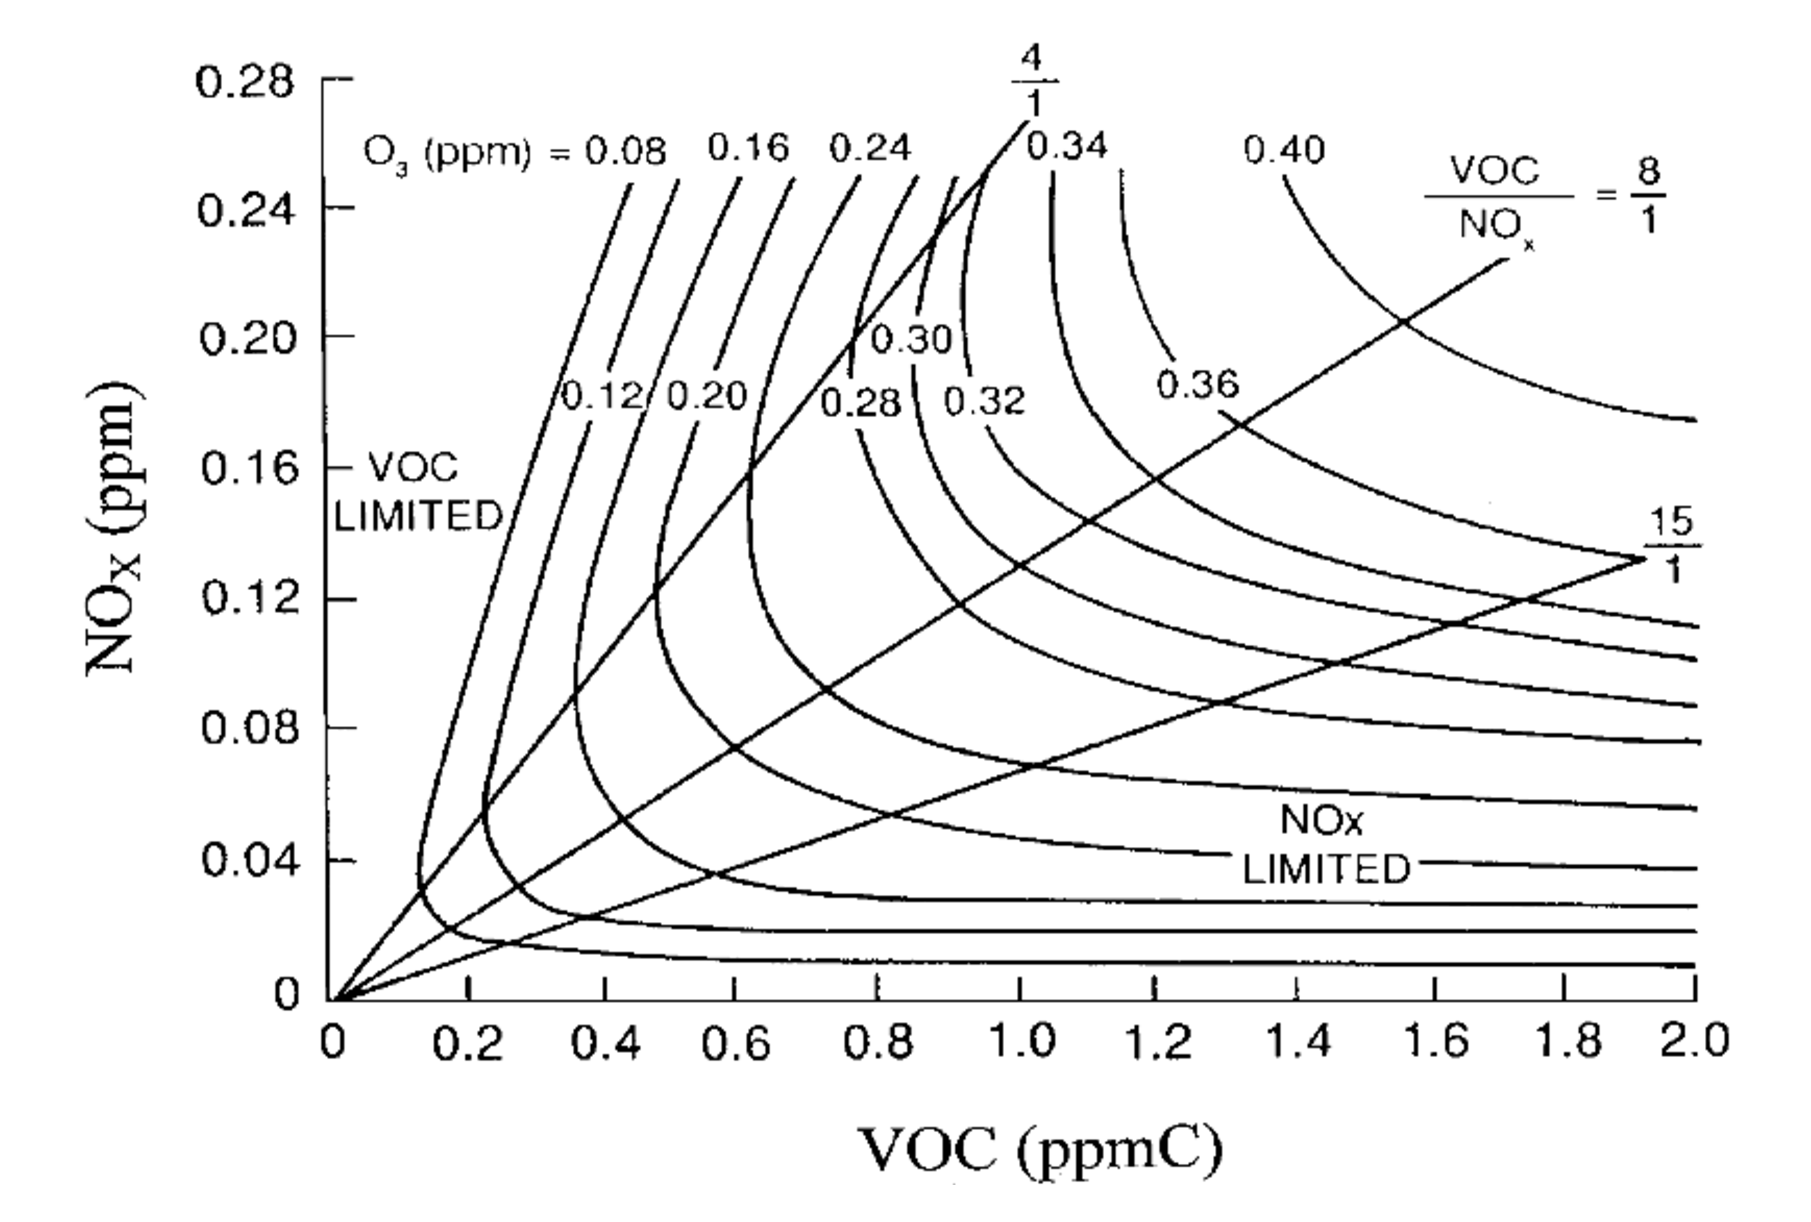
\includegraphics[width = 0.9\textwidth]{O3_isopleth}%
		\label{f:O3_isopleth}%
	\end{center}%
\end{figure}%
%balance of NOx & NMVOC for O3 production
The fate of peroxy radicals produced during VOC degradation depends on the ratio of the concentrations of radicals and \ce{NO_x} \citep{Kleinman:1991, Kleinman:1994}.
In regions with low-\ce{NO_x} concentrations, \ce{RO2} are more likely to react with other radicals rather than convert NO to \ce{NO2} leading to ozone production.
%The most common reactions are bimolecular destruction \eqref{r:HO2_OH}, which removes radicals, or combination of radicals \eqref{r:RO2_HO2} into reservoir species that may re-release radicals.
This is \emph{\ce{NO_x}-limited} chemistry.

On the other hand, reactions between radicals and \ce{NO_x} in regions with high levels of \ce{NO_x} are more likely to occur.
The production of \ce{HNO3} increases through \eqref{r:NO2_OH} removing OH and \ce{NO_x}.
This is \emph{VOC-limited} or \emph{\ce{NO_x}-saturated} chemistry.

The chemistry in low-\ce{NO_x} and high-\ce{NO_x} conditions indicates that ozone production is a non-linear process.
Figure~\ref{f:O3_isopleth}, from \citet{Jenkin:2000}, depicts the non-linear relationship between ozone as a function of VOC and \ce{NO_x}.
This relationship can be divided into distinct regimes of ozone production: \emph{\ce{NO_x}-sensitive} (or \emph{\ce{NO_x}-limited}), \emph{\ce{NO_x}-saturated} (or \emph{VOC-limited}) and \emph{VOC-and-\ce{NO_x}-sensitive} regimes. 

In the \ce{NO_x}-sensitive regime, increasing \ce{NO_x} increases the number of NO to \ce{NO2} conversions by peroxy radicals leading to ozone production.
However, increasing VOC levels has little effect on \ce{O3} production due to increased radical-radical reactions.

The \ce{NO_x}-saturated regime corresponds to high \ce{NO_x} concentrations where radicals tend to react with \ce{NO_x}. 
Increasing levels of VOC increase the likelihood of \ce{RO2} converting NO to \ce{NO2} leading to ozone production.
Increasing \ce{NO_x} levels will not increase \ce{O3} production.

The VOC-and-\ce{NO_x}-sensitive regime (contour ridges in Fig.~\ref{f:O3_isopleth}) is characterised by \ce{O3} production being sensitive to both VOC and \ce{NO_x} levels. 
Morever, it is in this atmospheric regime that the maximum amount of ozone is produced.
\citet{Kleinman:1994} showed that this non-linear relationship can be thought of as a titration process between radicals and \ce{NO_x} with the VOC-and-\ce{NO_x}-sensitive regime being the turning point.

The non-linear nature of ozone production is one of the challenges in controlling ozone levels.
The difficulty is exacerbated by the fact that the troposphere can alternate between these regimes depending on the meteorological conditions.
Moreover, fresh emissions tend to occur in \ce{NO_x}-saturated areas before being transported to VOC-and-\ce{NO_x}-sensitive and \ce{NO_x}-sensitive regions.

\subsection{Representing Atmospheric Chemistry in Models} \label{ss:chemistry_models}
Representing the degradation chemistry for each VOC in a chemical transport model (CTM) is unrealistic.
Even if all the secondary degradation pathways and products were known for every VOC, a CTM is unable to efficiently numerically solve the differential equations.

The representation of atmospheric chemistry in a CTM is called a chemical mechanism.
Chemical mechanisms are developed by simplifying and aggregating VOCs, degradation products and reactions.
Less aggressive simplification approaches may result in a chemical mechanism having thousands of species while more aggressive simplification may result in only a hundred species. 
Chemical mechanisms are verified by comparing the concentrations of field studies or controlled chamber study experiments to model simulations \citep{Stockwell:2012}.
Section~\ref{s:chemical_mechanisms} includes further details of the simplification techniques used to develop chemical mechanisms.

Chemical mechanism comparison studies, such as \citet{Kuhn:1998} and \citet{Emmerson:2009}, compare the outputs of different chemical mechanisms using the same model setup and initial conditions.
These studies showed that the differences in representing atmospheric chemistry can lead to large differences in simulated ozone concentrations.
These comparisons of the concentrations of key atmospheric species (such as ozone, OH and \ce{NO_x}) indicate that the chemical mechanisms leads to differences but does not help in pointing out the root cause.

Determining the source of differences between chemical mechanisms is a difficult task due to the interlinked chemistry of many key species.
As part of this study, the ozone production from different chemical mechanisms is compared and differences in the treatment of VOC degradation chemistry is determined.
The research questions driving this comparison are presented in Sect.~\ref{s:research_questions} and the results are described in Sect.~\ref{s:chemical_mechanism_results}.

\section{Source and Sinks of Ozone Precursors} \label{s:precursor_emissions}
%temporal profile of emissions
Ozone precursors are emitted from many anthropogenic and biogenic sources with varying emissions throughout the year, month or time of day.
In many regions, reduced road transport during the weekend leads to a noticible reduction in \ce{NO_x} emissions influencing ozone levels.
This is called the ``weekend-effect''.
For example, ozone production is \ce{NO_x}-saturated during weekdays in San Joaquin Valley, California but during the weekend higher ozone levels are recorded as the reduction in \ce{NO_x} levels leads to VOC-and-\ce{NO_x}-sensitive chemistry \citep{Pusede:2014}.
Many sources of NMVOC, such as industry and solvent use, also reduce activities during the weekend.
Residential combustion is highest during the winter months and lowest during the summer \citep{Gon:2011}.

% NOx sources and quantities, weekend effect
\subsection[NOx]{\ce{NO_x}}
Anthropogenic activities are the main source of \ce{NO_x} emissions into the atmosphere.
In the year 2000, almost $52$~Tg~N were emitted with 65~\% through fossil fuel combustion \citep{Seinfeld:2006}. 
Examples of fossil fuel combustion emitting \ce{NO_x} are transportation using diesel or petrol vehicles, industrial activities and domestic heating \citep{vonSchneidemesser:2015}.

Up to $95$~\% of \ce{NO_x} emissions from combustion are emitted as NO, which is oxidised to form \ce{NO2} through \eqref{r:NO_O3} and \eqref{r:HO2_NO}.
However, due to the increase in diesel vehicles and the implementation of diesel filters the fraction of emitted \ce{NO2} from vehicles has increased.
\citet{Grice:2009} showed that over Europe, emissions of \ce{NO2} from diesel vehicles have increased from $8.6$~\% in 2000 to $12.4$~\% in 2004.

Despite the majority of \ce{NO_x} emissions coming from human activities, there are also natural sources of \ce{NO_x}.
Lightning is an important source of \ce{NO_x} in the free troposphere while emissions of \ce{NO_x} from soils are important in remote regions with little anthropogenic influence.
Lightning and soils each contributed $\sim$~$10$~\% to global \ce{NO_x} emissions in 2000 \citep{Seinfeld:2006}.

The main sink of \ce{NO_x} is through deposition of nitric acid, formed via \eqref{r:NO2_OH}.
Temporary reservoirs, such as peroxy nitrates and HONO, may be transported away from sources into areas devoid of large sources of \ce{NO_x}.
These sources and sinks of \ce{NO_x} are illustrated in Fig.~\ref{f:NOx_sources_sinks}.
\begin{figure}[t]%
	\begin{center}%
        \caption[\ce{NO_x} sources and sinks]{The sources and sinks of \ce{NO_x}, adapted from \citet{Seinfeld:2006}.}%
        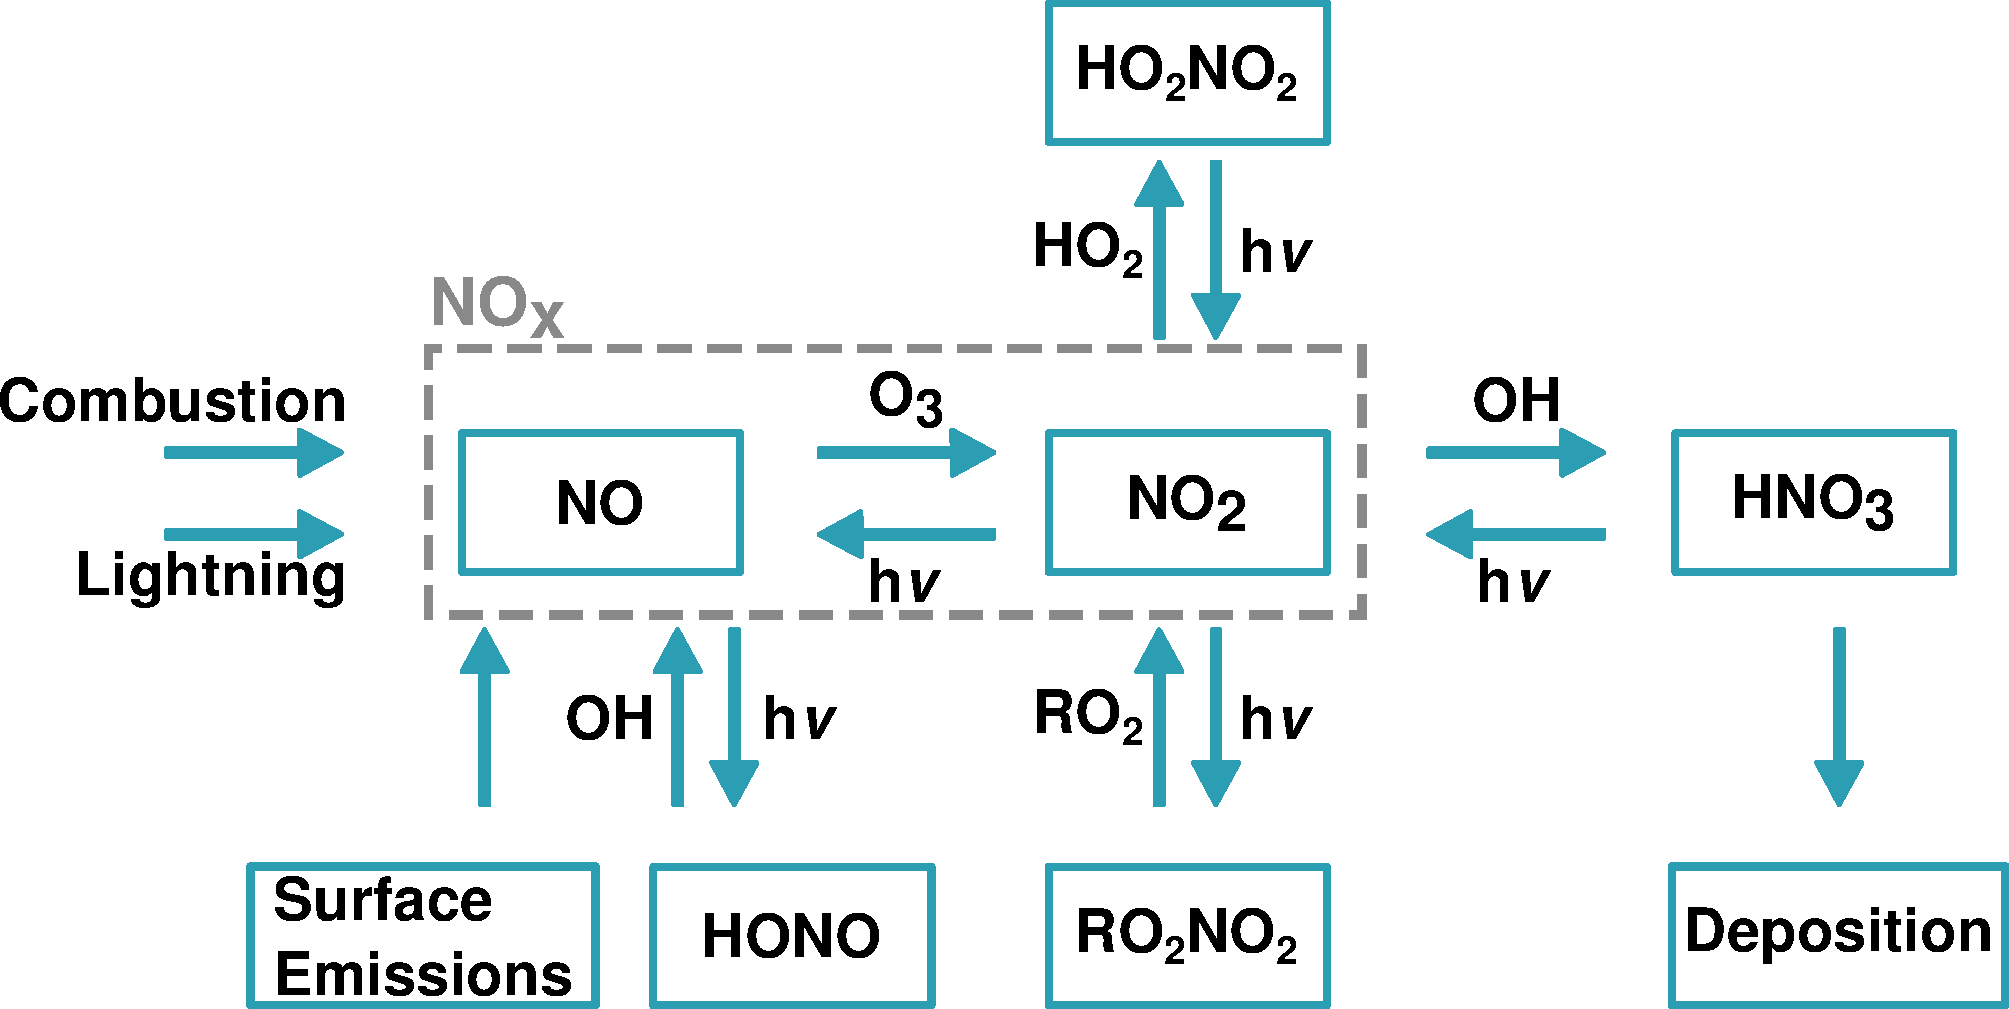
\includegraphics[width = \textwidth]{NOx_sources_sinks}%
        \label{f:NOx_sources_sinks}%
	\end{center}%
\end{figure}%

\subsection{VOCs}
The main sink of VOCs is the oxidation chemistry described in Sect.~\ref{s:ozone_chemistry}.
The degradation of a VOC yields the maximum possible amount of ozone when every peroxy radical converts NO to \ce{NO2} called the \emph{ozone production potential} (OPP) of a VOC.
In reality, the OPP of a VOC is never achieved as other reactions with peroxy radicals occur however the OPP is useful for assessing the amount of ozone produced from emitted VOCs.

\subsubsection{Carbon Monoxide}
Carbon monoxide is emitted directly into the troposphere through combustion and industrial processes.
An equally-important source of CO is its formation during the degradation of VOCs.
\citet{Hauglustaine:1998} estimated that $881$~Tg~yr$^{-1}$ of CO was produced globally from chemical oxidation of VOC while $1219$~Tg~yr$^{-1}$ of CO was directly emitted.

The reaction between CO and OH \eqref{r:CO_OH} is the main sink of CO.
The OPP of CO is one as the degradation of CO produces one peroxy radical (\ce{HO2}), thus a maximum of one molecule of ozone may be produced during CO degradation.

\subsubsection{Methane}
Emissions of methane range between $500$ and $600$~Tg~\ce{CH4}~yr$^{-1}$ with $\sim$~$60$~\% of the emissions from anthropogenic sources.
The main anthropogenic sources of \ce{CH4} are agriculture, fossil fuels and biomass burning with agriculture contributing $60$~\% of the anthropogenically emitted \ce{CH4}.
Emissions from wetlands are the main natural source of methane emissions \citep{Kirschke:2013}.

Methane has a lifetime of about $9$~years, significantly longer than other VOCs.
Thus, methane influences ozone production on the global rather than the regional scale.  

Reaction with OH \eqref{r:CH4_OH} is the main sink of methane and the secondary degradation of \ce{CH4} (Fig.~\ref{f:CH4_oxidation}) produces CO and four peroxy radicals ($1 \times$ \ce{CH3O2}, $3 \times$ \ce{HO2}).
Thus the OPP of methane is five as methane degradation can produce a maximum five molecules of \ce{O3} per molecule of \ce{CH4} oxidised. 

\subsubsection{NMVOCs}
%VOCs, types of VOCs and source (A vs B)
A wide variety of NMVOCs are emitted from anthropogenic activities directly into the troposphere.
Solvent use, industry, fossil fuel burning and transportation are all major activities emitting NMVOCs of varying functional groups, carbon numbers and reactivity.
Emissions of NMVOC from vegetation depends on meteorological variables (such as, temperature and radiation) and biological variables (such as, leaf age and leaf area index) \citep{Guenther:2012}.

\citet{Lamarque:2010} estimated that in 2000, $130$~Tg~NMVOC were globally emitted from anthropogenic sources.
This amount is dwarfed by emissions from biogenic sources -- $1000$~Tg~NMVOC~yr$^{-1}$ \citep{Guenther:2012}.
Isoprene (\ce{C5H8}) emitted from vegetation dominates at the global scale however emissions of monoterpenes and sesquiterpenes from vegetation may also be significant.

Although isoprene is considered as a biogenic VOC (BVOC), it has been measured in the urban areas of London and Paris away from biogenic emission sources.
Transport of isoprene is unlikely as isoprene is a highly reactive NMVOC indicating anthropogenic sources of isoprene \citep{vonSchneidemesser:2011}.
Other NMVOC emitted from anthropogenic sources, such as methanol and acetaldehyde, are also emitted from vegetation \citep{Guenther:2012}.

The maximum number of molecules of \ce{O3} produced per degradation of an emitted NMVOC depends on the type and the number of carbons of the NMVOC leading to a wide range of OPPs for different NMVOC.
Unsaturated NMVOC, such as alkenes, tend to have larger OPPs than alkanes (saturated NMVOC).
Even within a functional group of NMVOC different OPPs are calculated.
For example, benzene and xylene are both aromatic compounds but as benzene is a more chemically stable molecule it has a lower OPP than xylene \citep{Carter:1994}.

OPPs for complex NMVOCs are calculated using models by incrementally varying the concentration of an NMVOC and calculating the change in ozone.
Different scales calculating the OPP of NMVOC have been developed using different \ce{NO_x} conditions.
The Maximum Incremental Reactivity (MIR) and Maximum Ozone Incremental Reactivity scales of \citet{Carter:1994} and the Tagged Ozone Production Potential (TOPP) are examples of OPP scales for NMVOCs.

\subsection{Representing NMVOC Emissions in Models}
%representation of VOC emissions in models using emission inventories
Emissions of NMVOC species are a critical input in models and emission inventories are used to specify the type and quantity of emissions from source categories.
Table~\ref{t:SNAP} lists the source sectors of emissions used by the TNO\_MACCIII emission inventory \citep{Kuenen:2014}.
Emission inventories are available for the global or regional emissions.
For example, EDGAR \citep{EDGAR:1996} specifies global emissions while TNO\_MACCIII \citep{Kuenen:2014} specifies european emissions.
\begin{table}[t]%
    \centering%
    \caption[Emission source sectors in the TNO\_MACCIII]{Emission source sectors for anthropogenic emissions listed in the TNO\_MACCIII inventory \citep{Kuenen:2014}.}%
    \begin{tabular}{ll}%
        \hline \hline
        \textbf{Description} & \textbf{Description} \\
        \hline \hline
        Public Power & Road Transport: Others \\
        Residential Combustion & Road Transport: Evaporation \\
        Industry & Road Transport: Wear \\
        Fossil Fuel & Non-road Transport \\
        Solvent Use & Waste \\
        Road Transport: Gasoline & Agriculture \\
        Road Transport: Diesel & \\ 
        \hline \hline
    \end{tabular}%
    \label{t:SNAP}%
\end{table}% 

Many uncertainties are associated with emission inventories.
For example, \citet{Coll:2010} showed that large discrepancies arise between ambient measurements and emission inventories.
Also, the temporal variation of emissions are not captured by emission inventories \citep{Boynard:2014}. 

BVOC emissions depend on meteorolgical and biological variables and lgorithms estimating BVOC emissions may be calculated as part of the model simulation instead of an emission inventory.
The Model of Emissions of Gases and Aerosols from Nature (MEGAN) \citep{Guenther:2006, Guenther:2012} calculates BVOC emissions at each model time-step using the temperature and radiation values determined from the model.
The choice of on-line algorithm or emission inventory to specify BVOC emissions influences modelled ozone concentrations. 
For example, \citet{Curci:2009} noted large differences in summertime ozone concentrations over Europe when using a gridded emission inventory or an on-line algorithm.

%emissions in models - lumping
%Uncertainties when using emission inventories arise as the speciation of emissions to individual chemical species or groups differs between emission inventories.
Emissions of the NMVOCs specified by an emission inventory are mapped to the chemical mechanism species used in the model.
This mapping is not standardised throughout the modelling community with the same NMVOC emissions possibly being allocated to different chemical species even if using the same chemical mechanism \citep{Carter:2015}.

The influence of the speciation of NMVOC emissions on modelled ozone production is determined as part of this work.
Moreover, the effect of using the same speciations of NMVOC emissions with different chemical mechanisms is also explored.
Section~\ref{s:research_questions} outlines the research questions and the results are presented in Sect.~\ref{s:EI_results}.

\section{Effects of Meteorology on Ozone Production} \label{s:meteo_ozone}
\begin{table}%
    \centering%
    \caption[Influence of meteorological variables on ozone production]{Influence of meteorological variables on ozone production, taken from \citet{Jacob:2009}.}%
    \begin{tabular}{ll}%
        \hline \hline
        \textbf{Meteorological Variable} & \textbf{Influence on Ozone} \\
        \hline \hline
        Temperature & Consistently positive \\
        Stagnation & Consistently positive \\
        Wind Speed & Generally negative \\
        Mixing Height & Weak or variable \\
        Humidity & Weak or variable \\
        Cloud Cover & Generally negative \\
        Precipitation & Weak or variable \\
        \hline \hline
    \end{tabular}%
    \label{t:meteo_vars}%
\end{table}%
%metereology impacts 
Meteorological conditions influence the production of ozone with clear and calm summer days typically having high ozone levels \citep{Duenas:2002}.
\citet{Comrie:1997} noted a complex relationship between meteorology and ozone due to competing positive and negative effects on ozone production.
Table~\ref{t:meteo_vars}, taken from \citet{Jacob:2009}, details the effects of specific meteorological variables on ozone production.

Climate change is predicted to influence many meteorological variables and increase the number of heatwaves.
Thus understanding the influence of meteorology on ozone production is particularly important for future predictions of air quality and tackling ozone pollution in a changing climate.

\subsubsection{Humidity}
Humidity influences ozone production both positively and negatively.
When \ce{O(^1D)}, originating from ozone photolysis \eqref{r:O3_hvb} reacts with water vapour \eqref{r:O1D_H2O}, the production of OH radicals leads to ozone loss.
However, the initiation of VOC degradation through reaction with OH can lead to ozone production (Sect.~\ref{s:ozone_chemistry}).
These competing effects of water vapour on ozone production lead to a weak correlation of ozone production with water vapour \citep{Jacob:2009}.

\subsubsection{Wind Speed}
High wind speeds transport ozone precursors away from their sources leading to a generally negative effect on ozone pollution over a region.
Model projections of \citet{Doherty:2013} showed that while climate change is expected to change large-scale atmospheric transport there is little influence on the spatial patterns of mean concentrations of ozone.

\subsubsection{Stagnation}
During periods of low wind speeds, emissions of ozone precursors remain close to their sources.
These stagnant conditions over polluted urban areas are highly correlated with increased ozone production over urban areas \citep{Jacob:2009}.
Heatwaves result from stagnant conditions along with high temperatures enhancing the ozone pollution over a region.

\subsubsection{Mixing Height}
The effects of the mixing height of the planetary boundary layer (PBL) with the free troposphere depend on the region.
For example, \citet{Dawson:2007} found that over the Eastern U.S., regions with low ozone are positively correlated with mixing height whereas regions with high ozone levels are negatively affected.
This spatial effect of mixing height on ozone production depends on the difference between ozone levels within the PBL and the free troposphere \citep{Jacob:2009}.

Mixing between the PBL and free troposphere into regions with levels of surface ozone lower than the free troposphere is an additional source of ozone.
Conversely, mixing of the elevated levels of ozone from polluted areas into the free troposphere reduces the surface ozone burden.

\subsubsection{Temperature}
Temperature is positively correlated with ozone in many areas.
\citet{Otero:2016} showed that temperature was the main driver of summertime ozone values over many areas of central Europe while \citet{Camalier:2007} correlated ozone with temperature over the Eastern US.
\citet{Sillman:1995a} illustrated that only ozone pollution produced from the chemistry described in Sect.~\ref{s:ozone_chemistry} is correlated with temperature rather than background ozone, the ozone levels without the influence of anthropogenic emissions.

Temperature directly influences ozone levels in two ways: increasing the emissions of VOCs from vegetation and speeding up the rates of chemical reactions.
The review of \citet{Pusede:2015} showed that the temperature dependence of radical production, organic reactivity, the shorter lifetime of \ce{RO2NO2} and the formation of alkyl nitrates \eqref{r:RO2_NOb} affects ozone production.

There is a lack of detailed process studies separating the direct effects of temperature on ozone over differing \ce{NO_x} conditions despite observational and regional modelling studies correlating temperature with ozone production. 
The final part of this work addresses whether the increase in BVOC emissions or faster reaction rates with temperature is more important for ozone production.
The research questions for this study are detailed in Sect.~\ref{s:research_questions} and results are presented in Sect.~\ref{s:T-O3_results}.

\section{Research Questions} \label{s:research_questions}
The detailed chemistry producing ozone cannot be fully represented in models for reasons of computational efficiency.
Thus models select a particular representation of atmospheric chemistry raising the overarching research questions for this thesis:
\begin{itemize}
    \item How do representations of detailed atmospheric chemistry influence simulated ozone production?
    \item What are the most important chemical processes when simulating ozone production?
\end{itemize}
This question is addressed through detailed modelling studies highlighting the chemical processes having the largest impact on simulated ozone production under three different conditions.

Firstly, different simplified versions of the ozone production chemistry are available to the modelling community with comparison studies showing that ozone concentrations vary between chemical mechanisms.
These chemical mechanism comparison studies do not determine the root causes of the differences between chemical mechanism, leading to the research questions:
\begin{itemize}
	\item How do the simplification techniques used by different chemical mechanisms affect ozone production? 
    \item Which processes are responsible for differences in ozone production with different chemical mechanisms?
\end{itemize}

Secondly, NMVOC emissions are a known source of uncertainty in modelling experiments.
The choice of emission inventory influences the speciation of individual NMVOC emissions possibly influencing ozone production.
By comparing the ozone produced using different emission inventories, the following research questions are addressed:
\begin{itemize}
	\item What is the influence on modelled ozone production when using different speciations of emitted NMVOCs? 
    \item Does this influence change when using different chemical mechanisms?
\end{itemize}

Finally, meteorology influences ozone production with temperature having the strongest positive correlation with ozone.
Temperature directly influences ozone production through increasing biogenic emissions and speeding up the reaction rates of chemical reactions.
\begin{itemize}
    \item Are temperature-dependent emissions or chemical processes more important for ozone production with increasing temperature? 
    \item How is the ozone-temperature relationship treated by different chemical mechanisms?
\end{itemize}

Detailed processed studies are performed using a box model to address these research questions, details of the experiments are presented in Chap.~\ref{c:methodology}.
The results of the experiments are found in Chap.~\ref{c:papers}, the general discussion and conclusions of the thesis are in Chap.~\ref{c:conclusions}.

\clearpage{\pagestyle{empty}\cleardoublepage}

\chapter{Methodology} \label{c:methodology}
This chapter details the methodology used to address the research questions of this work (Sect.~\ref{s:research_questions}).
A brief description of AQ modelling is followed by the model set-up used in the separate studies (Sect.~\ref{s:modelling}). 
The chemical mechanisms used in this work are introduced in Sect.~\ref{s:chemical_mechanisms} and the required initial and boundary conditions are described in Sect.~\ref{s:initial_conditions} 

\section{Air Quality Modelling} \label{s:modelling}
AQ models are mathematical representations of the atmosphere designed to produce continuous output fields that aid in explaining sources of air pollution.
All models numerically solve the system of differential equations describing the conservation of chemical species used by the model \citep{Russell:2000}.

Solving the system of differential equations requires initial and boundary conditions for each chemical species.
Initial conditions fix the starting concentrations of each species in every grid-box.
Boundary conditions require knowledge of the concentration and transport of each species at the boundary edges of the model grid.

Eulerian models are the most common type of AQ model \citep{Russell:2000}.
These models describe the atmosphere by fixed grid-boxes where species are transported in and out of the boxes \citep{Seinfeld:2006}. 
Box models are the simplest type of model (zero-dimensional) having uniform atmospheric concentrations that are a function of time.
Whereas 3-D models describe atmospheric concentrations as a function of time, latitude, longitude and height requiring more computing power than a box model \citep{Seinfeld:2006}.
Box models may lack realism but are useful for studying detailed processes influencing air quality.

\subsection{Model Description and Setup} \label{ss:model_setup}
The MECCA (Module Efficiently Calculating the Chemistry of the Atmosphere) box model was used throughout this work.
MECCA was developed by \citet{Sander:2005} and adapted to include MCM~v3.1 chemistry by \citet{Butler:2011}.
MECCA was used in the published studies of \citet{Kubistin:2010} and \citet{Lourens:2016}.

MECCA is written in Fortran code and runs on UNIX/Linux platforms.
The Kinetic Pre-Processor (KPP, \citet{Damian:2002}) processed the chemical mechanism and generated Fortran code further compiled within MECCA.
KPP has many choices of numerical solver for solving the differential equations, a Rosenbrock solver (ros3 option) was used throughout this work.

Emissions of species into the box and deposition of species out of the box were handled by KPP.
The chemical mechanism included pseudo-unimolecular reactions specifying the emissions and dry deposition of chemical species with the relevant rate.
The emitted chemical species and emission rates were read into the model using a namelist file.  
Namelist files also specified the initial and boundary conditions of chemical species.

\begin{table}[t]%
    \begin{center}%
        \caption{MECCA box model settings.}%
        \begin{tabular}{ll}%
            \hline \hline
            \textbf{Model Parameter} & \textbf{Setting} \\
            \hline \hline
            Pressure & $1013$ hPa \\
            Relative Humidity & $81$ \% \\
            Starting Date and Time & 27th March 06:00 \\
            Model Time Step & $20$ mins \\
            \hline \hline
        \end{tabular}%
        \label{t:model_setup}%
    \end{center}%
\end{table}%
The physical parameters used in MECCA throughout this work are detailed in Table~\ref{t:model_setup}.
In the first two studies, temperature was held constant at $293$~K ($20$\degree C) and the boundary layer height was fixed at $1000$~m.
In the final study, MECCA was updated to include a variable diurnal boundary layer height and temperature was systematically varied between $288$ and $313$~K ($15$--$40$~\degree C).
These changes to the model setup for the final study are outlined in Paper~III (Chap.~\ref{c:paper_3}).

Photolysis rates were paramaterised as a function of the solar zenith angle based on the approach of the MCM \citep{Jenkin:1997}.
This paramaterisation utilises the degree of latitude and in the first two studies $34$~\degree N, roughly the city of Los Angeles, was used.
In the final study, the latitude was set to $51$~\degree N simulating central European conditions.

\section{Chemical Mechanisms} \label{s:chemical_mechanisms}
\begin{table}[t]%
    \begin{center}%
        \caption{Chemical mechanisms used in this work.}%
        \scalebox{.85}[.85]{\begin{tabular}{lll}%
                \hline \hline
                \textbf{Chemical Mechanism} & \textbf{Lumping Type} & \textbf{Reference} \\
                \hline \hline
                \multirow{3}{*}{MCM v3.1 and v3.2} & \multirow{3}{*}{No lumping} & \citet{Jenkin:1997}, \citet{Jenkin:2003} \\
                & & \citet{Saunders:2003}, \citet{Bloss:2005} \\
                & & \citet{MCM_Site} \\
                CRIv2 & Lumped intermediate & \citet{Jenkin:2008} \\
                MOZART-4 & Lumped molecule & \citet{Emmons:2010} \\
                RADM2 & Lumped molecule & \citet{Stockwell:1990} \\
                RACM & Lumped molecule & \citet{Stockwell:1997} \\
                RACM2 & Lumped molecule & \citet{Goliff:2013} \\
                CBM-IV & Lumped structure & \citet{Gery:1989} \\
                CB05 & Lumped structure & \citet{Yarwood:2005} \\
                \hline \hline
            \end{tabular}%
        }%
        \label{t:mechanisms}%
    \end{center}%
    %\vspace{-13mm}
\end{table}%
The chemical mechanisms used in this study are listed in Table~\ref{t:mechanisms} with more details found in Paper~I (Sect.~\ref{s:chemical_mechanism_results}).
These chemical mechanisms were chosen as they are commonly used by the AQ modelling community as outlined by the review of European modelling groups by \citet{Baklanov:2014}.

The Master Chemical Mechanism (MCM, \citet{Jenkin:1997, Jenkin:2003, Saunders:2003, Bloss:2005, MCM_Site}) is a near-explicit chemical mechanism with a high level of detail making it ideal as the reference chemical mechanism in each study of this work.
The Common Representative Intermediates (CRI) chemical mechanism \citep{Jenkin:2008} is a lumped-intermediate mechanism where the degradation productions are aggregated (lumped) rather than emitted VOC.

Lumped molecule chemical mechanisms aggregate primary VOC into mechanism species and is the most commonly used simplification technique.
The lumped-molecule chemical mechanisms used in this work were Model for OZone and Related chemical Tracers (MOZART, \citet{Emmons:2010}), Regional Acid Deposition Model (RADM2, \citet{Stockwell:1990}), Regional Atmospheric Chemistry Mechanism (RACM, \citet{Stockwell:1997}) and RACM2 \citet{Goliff:2013}.
Lumped structure chemical mechanism represent emissions of NMVOC through emissions of mechanism species representing the bonds present in the NMVOC.
The Carbon Bond mechanisms CBM-IV \citep{Gery:1989} and CB05 \citep{Yarwood:2005} were the lumped-structure chemical mechanisms used in this work.

\subsection{Implementing Chemical Mechanisms in MECCA} \label{s:mechanisms_MECCA}
Each chemical mechanism listed in Table~\ref{t:mechanisms} was adapted to the KPP format used in the MECCA box model.
The WRF-Chem model \citep{Grell:2005} includes KPP versions of RADM2, RACM and CBM-IV and this was the source for these chemical mechanisms.
The full version of the CRI~v2 was obtained from \mbox{\url{http://mcm.leeds.ac.uk/CRI}} while the original reference was the source for all other chemical mechanisms in Table~\ref{t:mechanisms}.

In order to focus on the differences in the representation of VOC degradation between the chemical mechanisms, a number of harmonisations between the chemical mechanisms were implemented.
For these harmonisations, the approaches used by the reference chemical mechanism (MCM~v3.2) were implemented in the reduced chemical mechanisms.
These changes are detailed in Paper~I (Chap.~\ref{c:paper_1}). 

\subsection{Tagging of Chemical Mechanisms} \label{s:tagging}
AQ models can be used to allocate the effects of different precursors or emission sources on ozone production.
For example, source removal studies perform separate model simulations with and without emissions from a sector to quantify the effect of the sector on ozone production, such as the quantification of megacity emissions on ozone production in \citet{Butler:2009}.
Tagging is another approach where the chemical mechanism includes additional chemical species labelled (tagged) with source information.
For example, \citet{Emmons:2012} tagged the MOZART-4 chemistry to attribute ozone production to emission sources of \ce{NO_x}.

In \citet{Butler:2011}, tagged VOC chemistry allows allocation of ozone production to emitted VOC.
Tagging involves labelling every organic degradation product produced during the degradation of a VOC with the name of the VOC.
This labelling is repeated for every degradation product until the final degradation products (\ce{CO2} and \ce{H2O}) are produced, thus every VOC has a separate set of reactions fully describing its degradation.
This tagging approach uses \ce{O_x} production as a proxy for \ce{O3} production and is only valid for \ce{NO_x}-limited and VOC-and-\ce{NO_x} sensitive chemistry not \ce{NO_x}-saturated conditions.
The \ce{O_x} family includes \ce{O3}, \ce{NO2}, \ce{O(^1D)}, \ce{O(^3P)}, \ce{NO3}, \ce{N2O5} and other species involved in fast production and loss cycles with \ce{NO2}.

All chemical mechanisms in Table~\ref{t:mechanisms} were tagged using the approach of \citet{Butler:2011}.
In the first study, the tagging approach was the basis for comparing the respresentations of VOC degradation chemistry and their effects on ozone production.
The second study used VOC-and-\ce{NO_x}-sensitive conditions and simulations using the tagged chemical mechanisms determined sources of differences in ozone production from the solvent sector emission inventories of Table~\ref{t:solvent_speciations}.
Variable \ce{NO_x} conditions were used in the third study hence using the tagging approach was not possible.
Thus all model simulations assessing the ozone-temperature relationship with different \ce{NO_x} conditions were performed with non-tagged versions of the chemical mechanisms.

\section{Initial and Boundary Conditions} \label{s:initial_conditions}
In all simulations of this work, methane (\ce{CH4}) was fixed to $1.75$~ppmv while carbon monoxide (CO) and \ce{O3} were initialised at $200$~ppbv and $40$~ppbv and then allowed to evolve freely.
The initial conditions for NMVOC emissions were held constant until noon of the first day of simulations to simulate a fresh emissions plume.

\subsubsection{NMVOC Initial Conditions} 
The initial conditions for NMVOC species differed in each experiment, a brief summary is given below and details are found in the respective publications (Chaps.~\ref{c:paper_1}--\ref{c:paper_3}).
The first study used the initial conditions of the Los Angeles simulation in \citet{Butler:2011} to determine the emissions needed for constant mixing ratios of the initial NMVOCs.
These emissions were mapped to the appropriate chemical species of each chemical mechanism in Table~\ref{t:mechanisms} keeping the amount of emitted NMVOC constant between model runs.

\begin{table}[t]%
    \begin{center}%
        \caption{The solvent sector emission inventories compared in this work.}%
        \begin{tabular}{lllP{5.2cm}}%
            \hline \hline
            \textbf{Speciation} & \textbf{Comment} & \textbf{Reference} \\ 
            \hline \hline
            TNO & European average &  \citet{Builtjes:2002} \\ 
            IPCC & Model Specific & \citet{Ehhalt:2001} \\ 
            EMEP & Model Specific & \citet{Simpson:2012} \\
            DE94 & Country Specific & \citet{Friedrich:2002} \\ 
            GR95 & Country Specific & \citet{Sidiropoulos:2007} \\ 
            GR05 & Country Specific & \citet{Sidiropoulos:2007} \\ 
            UK98 & Country Specific & \citet{Goodwin:2000} \\ 
            UK08 & Country Specific & \citet{Murrells:2010} \\ 
            \hline \hline
        \end{tabular}%
        \label{t:solvent_speciations}%
    \end{center}%
    \vspace{-7mm}
\end{table}%
The second study used NMVOC emissions specified by the emission inventories for the solvent sector listed in Table~\ref{t:solvent_speciations} over a theoretical urban area of $1000$~km$^2$ with total NMVOC emissions of $1000$~tons/day.
The solvent sector contributes $\sim43$~\% by mass of total emissions \citep{AQEU:2011}, thus total NMVOC emissions of $430$~tons/day were used.
Further simulations used emissions from all other sectors (remaining $570$~tons/day) while varying the solvent sector NMVOC emissions.
Additional simulations included BVOC emissions of isoprene and monoterpenes while varying the speciation of NMVOC emissions from the solvent sector.

The NMVOC emissions of the solvent sector were assigned to MCM~v3.2 species based on the speciations of each emission inventory.
Model simulations were repeated using MOZART-4 and RADM2 to investigate whether changing the chemical mechanism affected the differences in ozone concentrations between the solvent sector emission inventories.

The final study looked at the ozone-temperature relationship over central Europe and used the emissions of NMVOC from Benelux (Belgium, Netherlands and Luxembourg).
The TNO\_MACCIII emissions for the year 2011 were used as anthropogenic NMVOC emissions and mapped to MCM~v3.2 species.
Temperature-independent emissions of biogenic species (isoprene and monoterpenes) were taken from the EMEP speciation \citep{Simpson:2012}.
Simulations using temperature-dependent emissions of isoprene used the MEGAN2.1 \citep{Guenther:2012} algorithm.
All simulations were repeated using the CRI~v2, MOZART-4, RADM2 and CB05 chemical mechanisms.

\subsubsection{\ce{NO_x} Initial Conditions} 
\ce{NO_x} conditions generating VOC-and-\ce{NO_x} sensitive chemistry were used in the first two studies.
This was achieved by emitting the amount of NO required to balance the source of radicals at each time step.
While the final study assessed the relationship between ozone and temperature with different \ce{NO_x} conditions.
For these simulations, a constant source of NO emissions was systematically varied between $5.0 \times 10^9$ and $1.5 \times 10^{12}$~molecules~(NO)~cm$^{-2}$~s$^{-1}$ at each temperature used in this study ($15$ -- $40$~\degree C).

\subsubsection{Boundary Conditions} 
No chemical boundary conditions were used in the first two studies as the experiments considered a contained box.
In the final study, MECCA included a diurnal profile of the PBL with vertical mixing into the free troposphere using the PBL heights from the BAERLIN2014 campaign \citep{Bonn:2016}.
The boundary conditions for the free troposphere mixing ratios for \ce{O3}, \ce{CH4} and CO were set to $50$~ppbv, $1.8$~ppmv and $116$~ppbv respectively. 
These mixing ratios were taken from the $700$~hPa height using the MATCH-MPIC chemical weather forecast data (\url{http://cwf.iass-potsdam.de/}) from March~21st, 2014.

\clearpage{\pagestyle{empty}\cleardoublepage}

\addtocontents{toc}{\protect\newpage}
\chapter{Presentation of Papers} \label{c:papers}
%% update section titles for TOC
This chapter outlines the main findings in each scientific papers published as part of this thesis.
These publications addressed the research questions framed in Sect.~\ref{s:research_questions}.

\singlespacing
\section[Paper 1]{Paper 1: A comparison of chemical mechanisms using tagged ozone production potential (TOPP) analysis} \label{s:chemical_mechanism_results}
\onehalfspacing

Published: \bibentry{Coates:2015}.
\vspace{5mm}

The first paper presents a box modelling study where the secondary chemistry represented in reduced chemical mechanisms (Table~\ref{t:mechanisms}) for VOC typical of urban environments (Table~2 of the article) were compared to the detailed MCM chemical mechanisms.
This paper verified how different simplification techniques of VOC degradation chemistry influenced ozone production and which processes were responsible for these differences in ozone production.

The degradation of each VOC prescribed in each chemical mechanism was ``tagged'' so that the \ce{O_x} production, a proxy for \ce{O3} production, could be attributed to the individual VOC source (Sect.~\ref{s:tagging}).
Tagging the chemical mechanisms involved labelling every organic degradation product from a VOC with the name of the emitted VOC, thus each VOC has a separate set of reactions fully describing its degradation until the final products, \ce{CO2} and \ce{H2O}, are produced.

The ozone mixing ratios using reduced chemical mechanisms were generally lower than the ozone mixing ratios using the reference MCM chemical mechanisms on the first two days of the simulations.
The VOC degradation prescribed in CRI~v2, a lumped-intermediate mechanism, produced the most similar amounts of \ce{O_x} to the MCM~v3.2 for each VOC.
Thus, the approach of using lumped-intermediate species whose degradation are based upon more detailed chemical mechanisms is preferable when developing future chemical mechanisms.

Many VOC are broken down into smaller-sized degradation products faster on the first day in reduced chemical mechanisms than the MCM~v3.2 leading to lower amounts of larger-sized degradation products that can further degrade and produce \ce{O_x}.
Thus, many VOC in reduced chemical mechanisms produce a lower maximum of \ce{O_x} than the MCM~v3.2 ultimately leading to lower \ce{O3} mixing ratios from the reduced chemical mechanisms compared to the MCM~v3.2.

Reactive VOC, such as unsaturated aliphatic and aromatic VOC, produce maximum \ce{O_x} on the first day of the simulations.
Unsaturated aliphatic VOC produce similar amounts of \ce{O_x} on the first day between mechanisms; differences in \ce{O_x} production arise when mechanism species are used to represent individual VOC.
Large inter-mechanism differences in \ce{O_x} production result from the degradation of aromatic VOC on the first day due to the faster break down of the mechanism species representing aromatic VOC in reduced chemical mechanisms.

The less-reactive alkanes produce maximum \ce{O_x} on the second day of simulations and this maximum is lower in each reduced chemical mechanism than the MCM~v3.2 due to the faster break down of alkanes into smaller sized degradation products on the first day.
The lower maximum in \ce{O_x} production during alkane degradation in reduced mechanisms would lead to an underestimation of the \ce{O3} levels downwind of VOC emissions, and an underestimation of the VOC contribution to tropospheric background \ce{O3} when using reduced mechanisms in regional or global modelling studies.

\todo[inline]{lumped-molecule vs lumped-struct, which processes}

\singlespacing
\section[Paper 2]{Paper 2: Variation of the NMVOC Speciation in the Solvent Sector and the Sensitivity of Modelled Tropospheric Ozone} \label{s:EI_results}
\onehalfspacing

Published: \bibentry{vonSchneidemesser:2016}.
\vspace{5mm}

The second publication compared the ozone levels produced when using different emission inventories of NMVOC emissions from the solvent sector within a box model.
Different chemical mechanisms (MCM~v3.2, MOZART-4 and RADM2) were also used to ascertain how different representations of the chemistry affects the ozone production using different emission inventories.

Emission inventories (EIs) are a critical model input but are also a major source of uncertainty in modelling studies.
Ambient measurements do not reflect the speciations of EIs in many locations, EIs may not adequately reflect the temporal nature of emissions and finally many EIs may be outdated.
Before taking upon the huge task of creating an EI addressing these issues, a scoping study looking at the effects of changing the model input from EIs on ozone production was started in this study.

The experimental setup was to consider solvent sector emissions, the emission sector with the single largest contribution to NMVOC, over an idealised urban area to scope out in an idealised nature how big the potential difference in ozone predications would be.
Model simulations used \ce{NO_x} conditions to simulate VOC-and-\ce{NO_x}-sensitive conditions thus looking at the differences in the maximum ozone amount of produced when using the emission inventories for the solvent sector in Table~\ref{t:solvent_speciations}.
Furthermore, as modelling groups use a range of models with different descriptions of VOC degradation chemistry, three chemical mechanisms were used that are typically used at the point (MCM~v3.2), regional (RADM2) and global (MOZART-4) scales.

A maximum difference of $15$~ppbv when using the different EIs was obtained from the box model simulations.
When using the same EI speciation, a maximum difference of $6.7$~ppbv was determined between simulations with different chemical mechanisms.
Thus both the choice of chemical mechanism and EI influenced the amount of ozone produced.

The tagging approach (Sect.~\ref{s:tagging}) used in Sect.~\ref{s:chemical_mechanism_results} was also applied and allowed allocation of \ce{O_x} production to the emitted NMVOC specified by each EI.
The first day production of \ce{O_x} was sensitive to the amount of reactive NMVOC, such as alkenes and aromatic, listed by the EI.
While the cumulative \ce{O_x} production after seven days was sensitive to the less-reactive NMVOC such as alkanes and oxygenated NMVOC.

Correlating the cumulative production of \ce{O_x} showed a positive correlation between \ce{O_x} production and the contribution of alkane species while a negative correlation was determined between \ce{O_x} production and contribution of oxygenated species.
EIs specifying more emissions of alkanes tended to have larger production of \ce{O_x} than EIs specifying larger emissions from oxygenated NMVOC.
Thus representing the contributions of these NMVOC influences the amounts of ozone produced during model simulations.

\singlespacing
\section[Paper 3]{Paper 3: The Influence of Temperature on Ozone Production under varying \ce{NO_x} Conditions -- a modelling study} \label{s:T-O3_results}
\onehalfspacing

Published: \bibentry{Coates:2016}.
\vspace{5mm}

The final study in this thesis looked at the ozone-temperature relationship with different \ce{NO_x} conditions in the box model.
The study aimed to determine whether temperature-dependent increases in reaction rates or isoprene emissions were more important on the urban scale.

Model simulations were performed using NMVOC emissions representative of central Europe, first using a temperature-independent source of isoprene emissions and then repeated with a temperature-dependent source of isoprene emissions.
The choice of chemical mechanism may also influence the relationship of temperature on ozone, thus all simulations were repeated with the MCM~v3.2, CRI~v2, MOZART-4, RADM2 and CB05 chemical mechanisms.

A non-linear relationship of ozone with temperature and \ce{NO_x} emissions was produced using each chemical mechanism. 
This non-linear relationship was similar to that previously reported from observational studies.

In each chemical mechanism, the increase in ozone with temperature was greater for temperature-dependent chemistry than for the increase in isoprene emissions with temperature.
The largest increases in ozone mixing ratios were obtained in High-\ce{NO_x} conditions and the lowest increase in ozone mixing ratios was achieved using Low-\ce{NO_x} conditions.

Analysis of \ce{O_x} budgets showed that the net increase in \ce{O_x} production with temperature was due to the faster reaction rates of initial oxidation of VOCs.
The faster reaction rates were mainly due to the increase of OH with temperature, related to the increase of \ce{O3} with temperature.
In the conditions of the box model, the faster oxidation of emitted VOC caused the increase of ozone with temperature.

Normalised \ce{O_x} production budgets were similar between chemical mechanisms.
Indicating that the differences in the ozone-temperature relationship between chemical mechanisms was due to the representation of VOCs or missing secondary degradation products.

The box model results were also compared to observational data and output from the 3-D model WRF-Chem.
The rate of increase of ozone with temperature from the box model was about half the rate of increase of ozone with temperature using observational and WRF-Chem output.
The lack of sensitivity in the box model was due to the experimental setup with a focus on instantaneous ozone production.
Whereas observational data and 3-D model such as WRF-Chem include further effects of temperature on ozone, such as stagnant conditions.
In stagnant conditions, high temperatures and low wind speeds lead to a build-up of ozone from previous days and these conditions were not considered in the experiments.

\clearpage{\pagestyle{empty}\cleardoublepage}

\chapter{Overall Discussion and Conclusions} \label{c:conclusions}
The research questions of Sect.~\ref{s:research_questions} were addressed by the box modelling studies of Chap.~\ref{c:papers} and these questions are answered in this chapter.
In each study the near-explicit MCM~v3.2 was the reference chemical mechanism with the simulations were repeated using reduced chemical mechanisms typically used by modelling groups for regional and global studies.

The first study compared the effects of different simplification techniques used by chemical mechanisms on ozone production.
The reduced chemical mechanisms used in the comparison were developed through lumping VOC degradation intermediates (CRI~v2), aggregating emitted NMVOCs into lumped molecules (MOZART-4, RADM2, RACM, RACM2) and expressing the emitted NMVOCs by lumped structure species (CBM-IV, CB05).
Out of these three simplification techniques, the lumped-intermediate approach produced the most similar amounts of ozone from each VOC to the MCM~v3.2 while the lumped-molecule and lumped-structure approaches generally produced less ozone than the MCM~v3.2 from the degradation of the VOC.
Thus the technique of lumping intermediate species rather than lumping VOCs appears promising for representing ozone production in future chemical mechanisms.

The second objective of the first study was to determine the processes responsible for the differences in ozone production using the different reduced chemical mechanisms.
The largest differences in ozone production from the reduced chemical mechanisms to the MCM~v3.2 were obtained for VOC represented by lumped mechanism species than those VOC explicitly represented.
In particular, the representation of aromatic VOC consistently produced lower ozone in all the reduced chemical mechanisms.
These differences in ozone production from aromatic VOC are not surprising as the degradation of aromatic VOC is an area of uncertainty \citep{Atkinson:2003}.
Even the detailed degradation chemistry of aromatic VOC in the MCM~v3.2 was unable to reproduce the results from chamber experiments \citep{Bloss:2005}.

Another process leading to lower ozone production from VOC degradation than the MCM~v3.2 was the faster break down of emitted VOC into smaller sized degradation products by lumped-molecule and lumped-structure chemical mechanisms.
In particular, the faster break down of alkanes in lumped-molecule and lumped-structure chemical mechanisms led to a lower peak of ozone production than the MCM~v3.2.
As alkanes are less-reactive VOC, they are more likely to be transported downwind of emission sources affecting ozone production in urban background areas.
Thus underestimating the ozone production from alkanes may impact simulated ozone levels of urban background areas.

The second study looked at the influence of varying the speciation of NMVOC emissions from the solvent sector on ozone production.
In box model experiments using the MCM~v3.2, differences in ozone production resulted from the different speciations of NMVOC emissions.
Ozone production on the first day was influenced by the amounts of alkenes and aromatic VOC specified by the solvent sector emission inventory (EI).
While the contribution of alkanes and oxygenated VOC by the solvent sector EI determined ozone production at the end of the simulations.

Similar differences in ozone production were obtained when repeating the box model simulations using reduced chemical mechanisms (MOZART-4, RADM2).
Thus although the emissions of NMVOC were represented by fewer species in the reduced chemical mechanisms than the MCM~v3.2, the differences in ozone production were not dampened by reducing the complexity of the chemical mechanism.

This study was designed as a scoping study to determine whether updating the speciation of an EI influenced model predictions of ozone levels.
Given the results of this study, further modelling studies using different atmospheric conditions and more complex models are warranted to obtain a complete picture of how varying the speciation of NMVOC emissions influences modelled ozone levels.

The final study modelled the relationship between ozone, temperature and \ce{NO_x} using central European conditions.
In order to verify whether temperature-dependent increases in reaction rates or isoprene emissions from nature are more important for the increase in ozone with temperature, separate simulations using a temperature-independent and temperature-dependent source of isoprene emissions were performed.
From these simulations, the absolute increase in ozone with temperature due to faster reaction rates was slightly higher than the increase in ozone with temperature due to increased isoprene emissions with temperature regardless of \ce{NO_x} conditions.
This result was surprising as studies (e.g. \citet{Racherla:2008}, \citet{Doherty:2013}) attributed the increase of ozone with temperature to increased isoprene emissions from vegetation.

The increase in ozone with temperature in all \ce{NO_x} conditions was principally due to the faster loss rates of the emitted VOC with temperature as the OH-reactivity of the emitted VOC increased with temperature.
As expected, peroxy nitrate (\ce{RO2NO2}) chemistry also played a role in the increase of ozone production with temperature with increased \ce{RO2NO2} decomposition at higher temperatures leading to more \ce{RO2} available to produce ozone.
Thus the initial oxidation of emitted VOC and \ce{RO2NO2} chemistry are critical to modelling the relationship between ozone, temperature and \ce{NO_x}.

Simulations were performed using reduced chemical mechanisms (CRI~v2, RADM2, MOZART-4, CB05) to determine whether the relationship between ozone, temperature and \ce{NO_x} differed between representations of atmospheric chemistry.
Each chemical mechanism reproduced the non-linear relationship between ozone, temperature and \ce{NO_x} with the choice of chemical mechanism not significantly changing this relationship.
The rate of increase of ozone with temperature was found to be more sensitive to the amount of mixing rather than the choice of chemical mechanism when comparing the box model simulations to observational and 3D model output.

Overall, the representation of detailed atmospheric chemistry influenced ozone production as in each of the studies differences between ozone levels were obtained when repeating model simulations with different chemical mechanisms.
Thus the choice of chemical mechanism is important for AQ modelling studies predicting future ozone levels.
The representation of emitted NMVOC by the different chemical mechanisms was critical leading to differences in ozone production in each study.
The secondary degradation processes of \ce{RO2NO2} chemistry and the rate of break down of emitted NMVOC by reduced chemical mechanisms also had implications for ozone production.

\clearpage{\pagestyle{empty}\cleardoublepage}

\chapter{Outlook} \label{c:outlook}
Although ozone pollution is a major problem in Europe, there is currently no legally binding limit value for ozone.
The EU Directive 2008/50/EG sets a target value for human health requiring the mean eight hourly ozone concentration not to exceed $120$~$\mu$g~m$^{-3}$ (= $60$~ppbv) on more than $25$ calendar days per year.
The same EU Directive also sets an AOT40 target value for the exposure of vegetation to ozone of less than $18,000$~$\mu$g~m$^{-3}\cdot$~h. 
AOT40 is the sum of the differences between the mean hourly ozone values above $80$~$\mu$g~m$^{-3}$ (= $40$~ppbv) and the value of $80$~$\mu$g~m$^{-3}$ between 8~am and 8~pm from May to July.

The EU has laws regulating the emissions of ozone precursors (\ce{NO_x} and VOC).
While these laws have reduced the emissions of both \ce{NO_x} and VOC over Europe, the target value for ozone is regularly exceeded throughout Europe.
The non-linear relationship between ozone, \ce{NO_x} and VOC as well as intercontinental transport of ozone and its precursors impact the response of ozone pollution despite reductions in precursor emissions.
The European Environmental Agency (EEA) recommends further mitigation efforts on the local, regional and global scales to reduce ambient ozone levels.

Setting a legally binding limit value for ambient ozone over Europe should inspire mitigation strategies at the local and regional scale in a bid to meet this limit.
Meeting a limit value requires assessing different mitigation approaches and here AQ modelling will be a vital tool in determining the efficacy of a mitigation strategy for reducing ambient ozone. 
Thus, research aiming to improve model performance would also aid in increasing the confidence of AQ predictions from models, an asset for judging different mitigation strategies.

\newpage
The detailed process studies performed as part of this work were designed to ultimately improve model performance increasing the confidence of the predictions of AQ models for mitigation strategies.
A number of recommendations to the AQ modelling community are listed below based on these studies.
AQ modelling groups should use up-to-date chemical mechanisms to incorporate the findings and recommendations from the chemical kinetics community as well as updated representations of emitted VOC and their secondary degradation.
This is undoubtably more work for a modelling group as further work such as testing the model with a new chemical mechanism and translating emissions into the new chemical species would need to be performed.
However, as shown in the first study, updated versions of the same chemical mechanism produced more similar amounts of ozone to the near-explicit MCM~v3.2 chemical mechanism.
Thus, using an updated chemical mechanism should increase the confidence of the modelled ozone production from the degradation of emitted VOCs.

As the lumped-intermediate chemical mechanism produced the most similar amounts of ozone to the MCM~v3.2, the approach of using a highly detailed chemical mechanism and lumping the degradation products appears promising for developing future chemical mechanisms.
This approach did not break down the emitted VOC into smaller degradation products as fast as the lumped-molecule and lumped-structure chemical mechanisms, which was the main cause for the lower ozone production using these chemical mechanisms compared to the MCM~v3.2.
Lumped-intermediate chemical mechanisms include more chemical species than lumped-molecule and lumped-structure chemical mechanisms making their use less appealling from a computational efficiency perspective.
However, gains in computational speed with modern computing centres might reduce this concern and facilitate the use of more complex chemical mechanisms as part of 3D models.

One aspect of future mitigation strategies could be to substitute the emissions of a more-reactive NMVOC, with a less-reactive NMVOC thus changing the NMVOC speciation profile from emission sectors.
Such mitigation strategies require updating emission inventories and assessing how the change in speciation could influence ambient ozone levels.
The results of the second study indicate that ozone production close to emission sources would be reduced using such mitigation strategies, but ozone production downwind may increase.

A warmer climate is predicted in the future as a result of climate change and this may affect ozone production chemistry in future emission scenarios.
The influence of meteorological variables on ozone production is extremely important with the third study demonstrating an increase in ozone production with temperature.
A deeper understanding of the effects of meteorology on ozone production is required to ensure that mitigation strategies are robust enough to still reduce ambient ozone in the future.

The increase of ozone with temperature was determined by the faster oxidation of the emitted NMVOC, further emphasising the importance of adequately representing both the speciation and initial degradation of emitted NMVOC.
The ozone-temperature relationship was sensitive to atmospheric mixing with less atmospheric mixing allowing the secondary degradation of NMVOC to proceed further than situations with enhanced atmospheric mixing.
This highlights the importance of representing the secondary degradation of NMVOC by the chemical mechanism used by an AQ model.

The results from the detailed process studies performed in this work were all performed using a box model and further work using 3D models is required to verify how additional processes, such as regional transport, also influence ozone production under these conditions.
The use of a box model was ideal for the scope of the studies of this thesis allowing a deeper insight into the chemical processes requiring a sharper focus than when using more realistic 3D models.
The recommendations of this thesis along with testing the sensitivity of ozone production within 3D models would aid in constructing effective mitigation strategies that would meet the EU regulations for ozone pollution.

\clearpage{\pagestyle{empty}\cleardoublepage}

\chapter{Summary and Zusammenfassung} \label{c:summary}
\vspace{-3mm}
\section{Summary}
\vspace{-3mm}
Tropospheric ozone is a short-lived climate forcing pollutant that is hazardous to human health and impacts deleteriously on vegetation.
Ozone is not emitted directly into the troposphere but formed from the photochemical reactions of VOCs and \ce{NO_x} with meteorological conditions strongly influencing ozone production.
This thesis assessed the chemical mechanisms of ozone production chemistry represented within air quality models by determining the influence of VOC degradation, the speciation of VOC emissions and temperature on modelled ozone production.
In order to focus on the impacts of the representation of tropospheric chemistry on ozone production, all modelling experiments in this work used a box model.
The highly-detailed MCM~v3.2 chemical mechanism was used as a reference and the model simulations were then repeated using reduced chemical mechanisms typically used by regional and global models.

The effects of different simplification approaches used by chemical mechanisms on ozone production were determined by comparing the ozone produced during VOC degradation between different chemical mechanisms.
The lumped-intermediate (CRI~v2) chemical mechanism produced the most similar amounts of ozone to the MCM~v3.2 from the degradation of each emitted VOC.
On the other hand, VOC degradation described by lumped-molecule (MOZART-4, RADM2, RACM and RACM2) and lumped-structure (CBM-IV and CB05) chemical mechanisms generally produced less ozone than the MCM~v3.2.
The lower ozone production from VOC degradation in the lumped-molecule and lumped-structure chemical mechanisms was caused by a faster breakdown of the emitted VOC into smaller sized degradation products.

The influence of the speciation of VOC emissions by an emission inventory on ozone production was established by comparing the ozone produced from different emission inventories of the solvent sector.
In these experiments, both the different emission inventories of VOC emissions and chemical mechanisms (MCM~v3.2, MOZART-4, RADM2) led to differences in peak ozone mixing ratios and ozone production.
These results indicated a sensitivity of ozone production to both the choice of chemical mechanism and emission inventory speciation.
The ozone production on the first day was influenced by the specified contributions of alkene and aromatic VOC.
Emission inventories specifying larger amounts of alkane emissions produced the largest amounts of ozone at the end of simulations than those specifying a larger contribution of emissions of oxygenated VOC.

The final study of this work considered the relationship between ozone, temperature and \ce{NO_x}.
The increase of ozone with temperature due to temperature-dependent chemistry was slightly larger than the increase of ozone with temperature due to temperature-dependent isoprene emissions in all \ce{NO_x}-conditions.
A non-linear relationship between ozone, temperature and \ce{NO_x} was obtained with each chemical mechanism used in this study (MCM~v3.2, CRI~v2, MOZART-4, RADM2 and CB05).
With each chemical mechanism, the temperature-dependent chemistry of VOC-oxidation and peroxy nitrates, such as PANs, caused the increase in ozone production with temperature.

The detailed process studies of this work will help improve model performance and the confidence in predictions of future ozone levels from air quality modelling studies.
The representation of VOC degradation and secondary processes, such as the rate of breakdown of the emitted VOCs and peroxy nitrate chemistry by a chemical mechanism, are particularly important processes for the predictions of ozone levels with different mitigation strategies.

%\newpage
\section{Zusammenfassung}
Troposphärisches Ozon ist ein kurzlebiger klimawirksamer Schadstoff, der für die menschliche Gesundheit gefährlich ist und sich auf schädliche Weise auf die Vegetation auswirkt.
Ozon wird nicht direkt in die Troposphäre emittiert, sondern entsteht aus den photochemischen Reaktionen von flüchtigen organischen Verbindungen (VOCs) und \ce{NO_x}, wobei meteorologische Bedingungen die Ozonproduktion stark beeinflussen.
In der vorliegenden Arbeit wurden verschiedene Chemiemechanismen zur Berechnung der Ozonproduktion in Atmosphären-Chemie-Modellen in Bezug auf den Einfluß des VOC-Abbaus, des Anteils verschiedener VOC-Komponenten an den VOC-Gesamtemissionen (\quotedblbase VOC Speciation``) und der Temperatur auf die modellierte Ozonproduktion untersucht.
Um detaillierte Prozessstudien mit einem Fokus auf die Repräsentativität der Auswirkung troposphärischer Chemie auf die Ozonproduktion in den Chemiemechanismen durchzuführen, wurden in dieser Arbeit Modellexperimente mit einem Box-Modell durchgeführt.
Als Referenz wurde zunächst der sehr detaillierte Chemiemechanismus MCM~v3.2 in Modellsimulationen verwendet.
Diese Simulationen wurden dann unter der Verwendung von reduzierten Chemiemechanismen, welche typischerweise von regionalen und globalen Modellen verwendet werden, wiederholt. 

Um die Auswirkungen der verschiedenen Vereinfachungsansätze, die in den Chemiemechanismen bezüglich der Ozonproduktion verwendet werden, auf die Ozonproduktion zu bestimmen, wurde die durch die verschiedenen Chemiemechanismen simulierte Ozonproduktion während des VOC-Abbaus verglichen.
Der Chemiemechanismus CRI~v2 mit zusammengefassten Zwischenprodukten (\quotedblbase lumped-intermediate``) hatte dabei im Vergleich zu  MCM~v3.2 die vergleichbarste Ozonmenge aus dem Abbau jedes emittierten VOC erzeugt. 
Der VOC-Abbau, welcher in den Chemiemechanismen mit zusammengefassten Molekülen (\quotedblbase lumped-molecule``) (MOZART-4, RADM2, RACM and RACM2) und zusammengefassten Strukturen (\quotedblbase lumped-structure``) (CBM-IV and CB05) beschrieben ist, produzierte jedoch gemeinhin weniger Ozon als MCM~v3.2. 
Die geringere Ozonproduktion während des VOC-Abbaus in den \quotedblbase lumped-molecule`` und \quotedblbase lumped-structure`` Chemiemechanismen wurde durch ein schnellerer Zerfall des emittierten VOC in kleinere Abbauprodukte verursacht.

Der Einfluss der \quotedblbase VOC Speciation`` von VOC-Emissionen durch ein Emissionsinventar wurde durch einen Vergleich des aus verschiedenen Emissionsinventaren des Lösungsmittelsektors produzierten Ozons festgestellt.
In diesen Experimenten führte die Verwendung unterschiedlicher VOC-Emissionsinventare und Chemiemechanismen (MCM~v3.2, MOZART-4, RADM2) zu Unterschieden bei den Spitzenwerten der Ozonmischungsverhältnisse sowie der Ozonproduktion.
Diese Ergebnisse zeigten eine Abhängigkeit der Ozonproduktion sowohl von der Wahl des Chemiemechanismus als auch von den \quotedblbase VOC Speciation`` in den Emissionsinventaren.
Am ersten Tag wurde die Ozonproduktion von den spezifizierten Beiträgen von Alken und aromatischen VOC beeinflusst.
Die Emissionsinventare mit höheren Mengen an Alkanemissionen erzeugten die größten Mengen an Ozon am Ende der Simulation, im Vergleich zu denen, die einen größeren Beitrag des Ausstoßes von oxygeniertem VOC definierten.

Die letzte Studie dieser Arbeit betrachtete die Beziehung zwischen Ozon, Temperatur und \ce{NO_x}.
Der Anstieg des Ozons mit der Temperatur aufgrund der temperaturabhängigen Chemie war geringfügig größer als der Anstieg des Ozons mit der Temperatur aufgrund der temperaturabhängigen Isoprenemissionen unter allen \ce{NO_x}-Bedingungen.
Ein nicht-linearer Zusammenhang zwischen Ozon, Temperatur und \ce{NO_x} wurde mit jedem in dieser Studie verwendeten Chemiemechanismus (MCM~v3.2, CRI~v2, MOZART-4, RADM2 und CB05) aufgezeigt.
Bei jedem Chemiemechanismus kam es aufgrund der temperaturabhängigen Chemie von VOC-Abbau und Peroxynitraten, wie z.~B. PANs, zu einem Anstieg der Ozonproduktion mit der Temperatur. 

Die detaillierten Prozessstudien dieser Arbeit werden dazu beitragen, die Güte von Modellen und das Vertrauen in die Prognosen zukünftiger Ozonwerte von Studien mit Atmosphären-Chemie-Modellen zu verbessern.
Die Darstellung des VOC-Abbaus und sekundärer Prozesse, wie der Zerfallgeschwindigkeit von emittierten VOCs sowie der Peroxynitratchemie durch einen Chemiemechanismus, sind besonders wichtige Prozesse für die Vorhersage der Ozonwerte unter Anwendung von unterschiedlichen Minderungsstrategien.

\clearpage{\pagestyle{empty}\cleardoublepage}

\fancyhead[LO,RE]{References}
\addcontentsline{toc}{chapter}{References}
\bibliographystyle{abbrvnat}
\bibliography{References} 
\clearpage{\pagestyle{empty}\cleardoublepage}

\chapter{Paper I: A comparison of chemical mechanisms using tagged ozone production potential (TOPP) analysis} \label{c:paper_1}
\clearpage{\pagestyle{empty}\cleardoublepage}
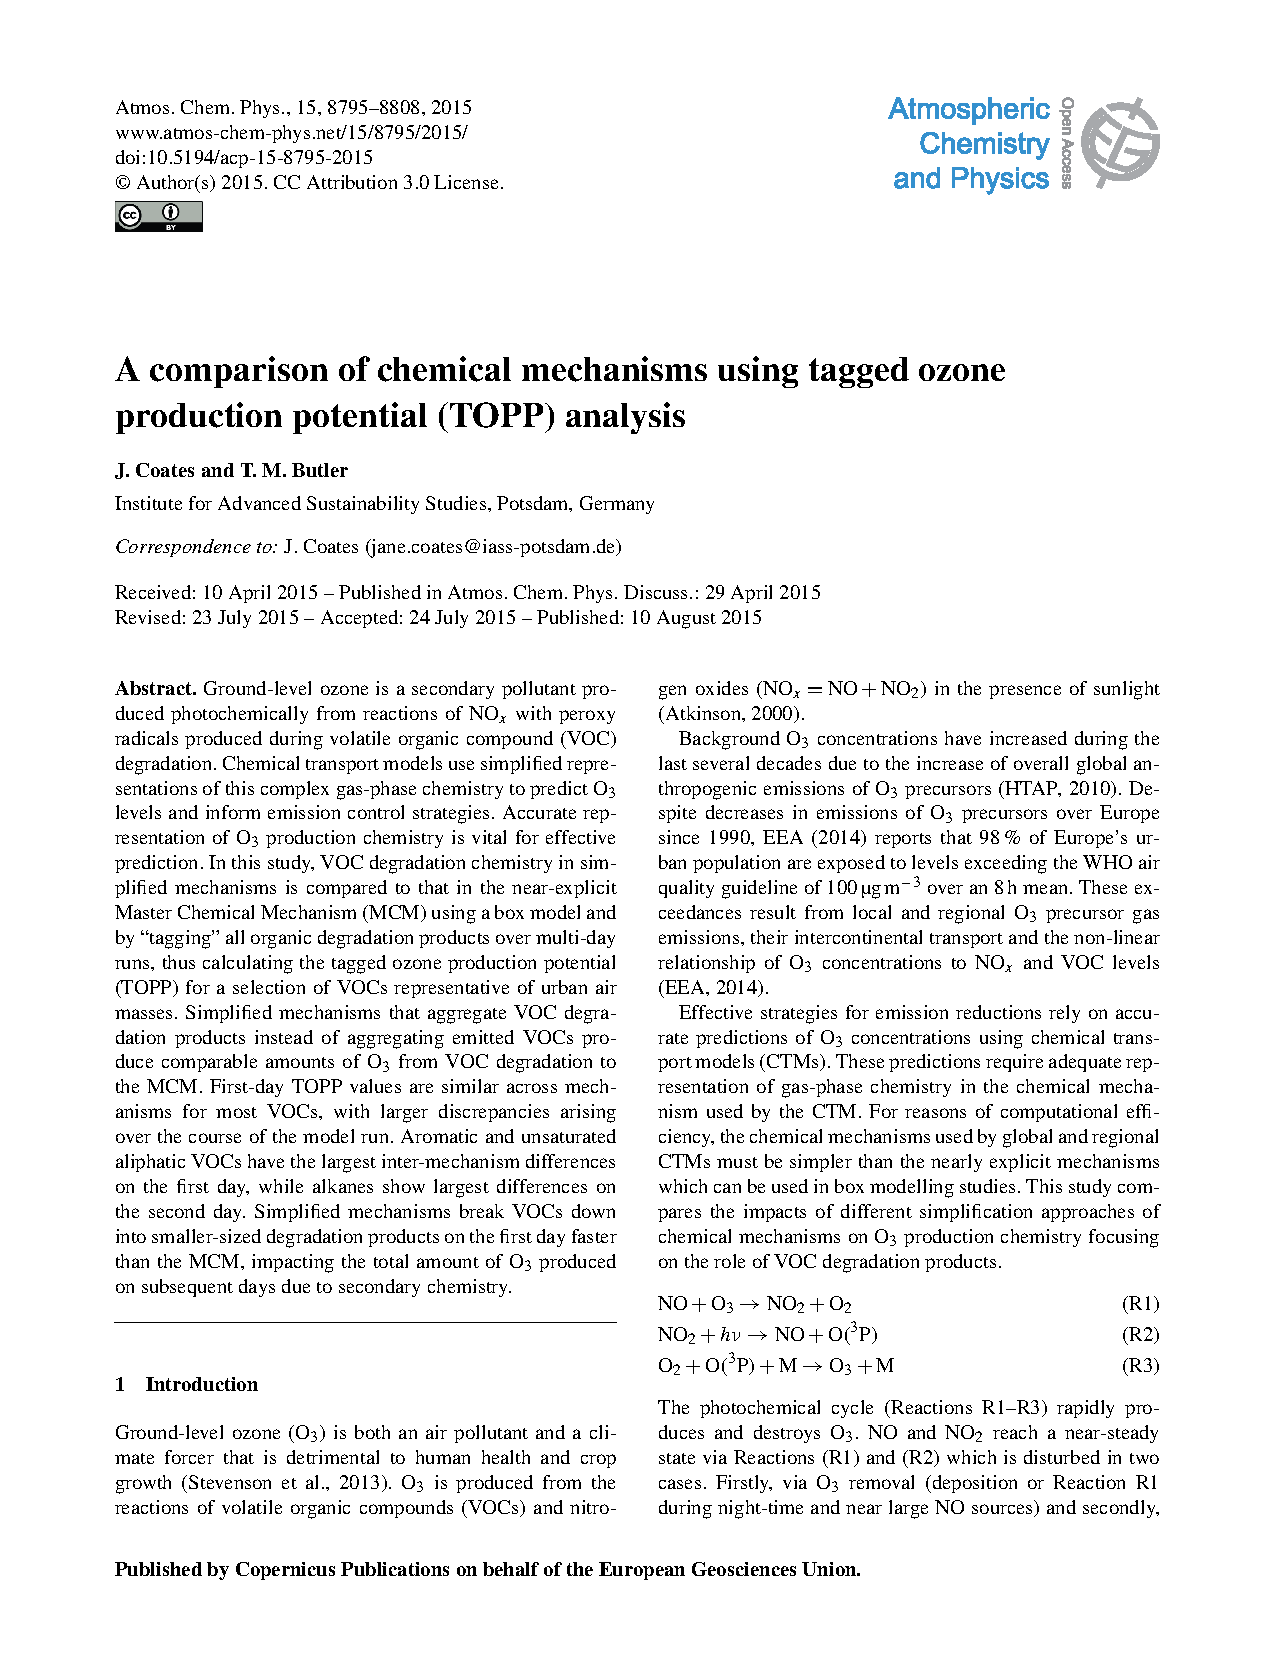
\includepdf[pages=-]{img/paper1.pdf}
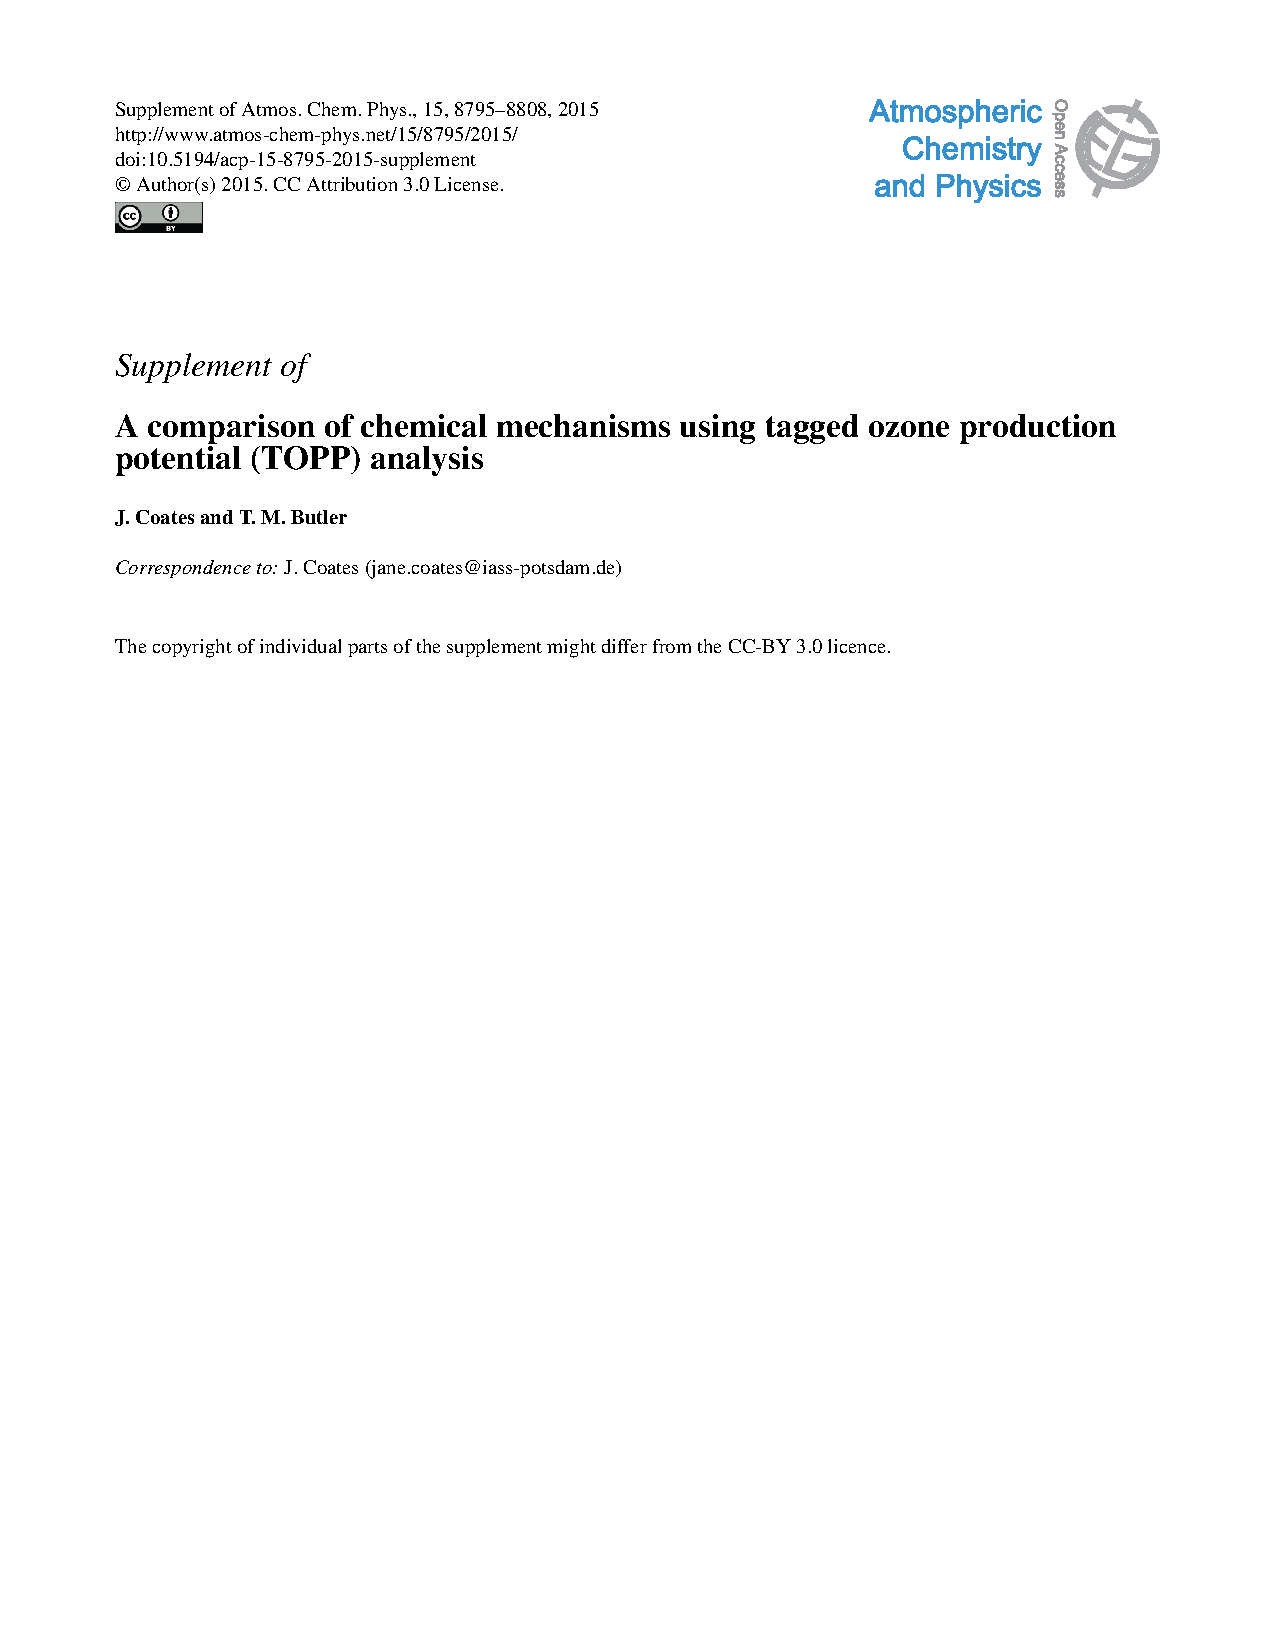
\includepdf[pages=-]{img/paper1-supplement.pdf}

\chapter{Paper II: Variation of the NMVOC Speciation in the Solvent Sector and the Sensitivity of Modelled Tropospheric Ozone} \label{c:paper_2}
\clearpage{\pagestyle{empty}\cleardoublepage}
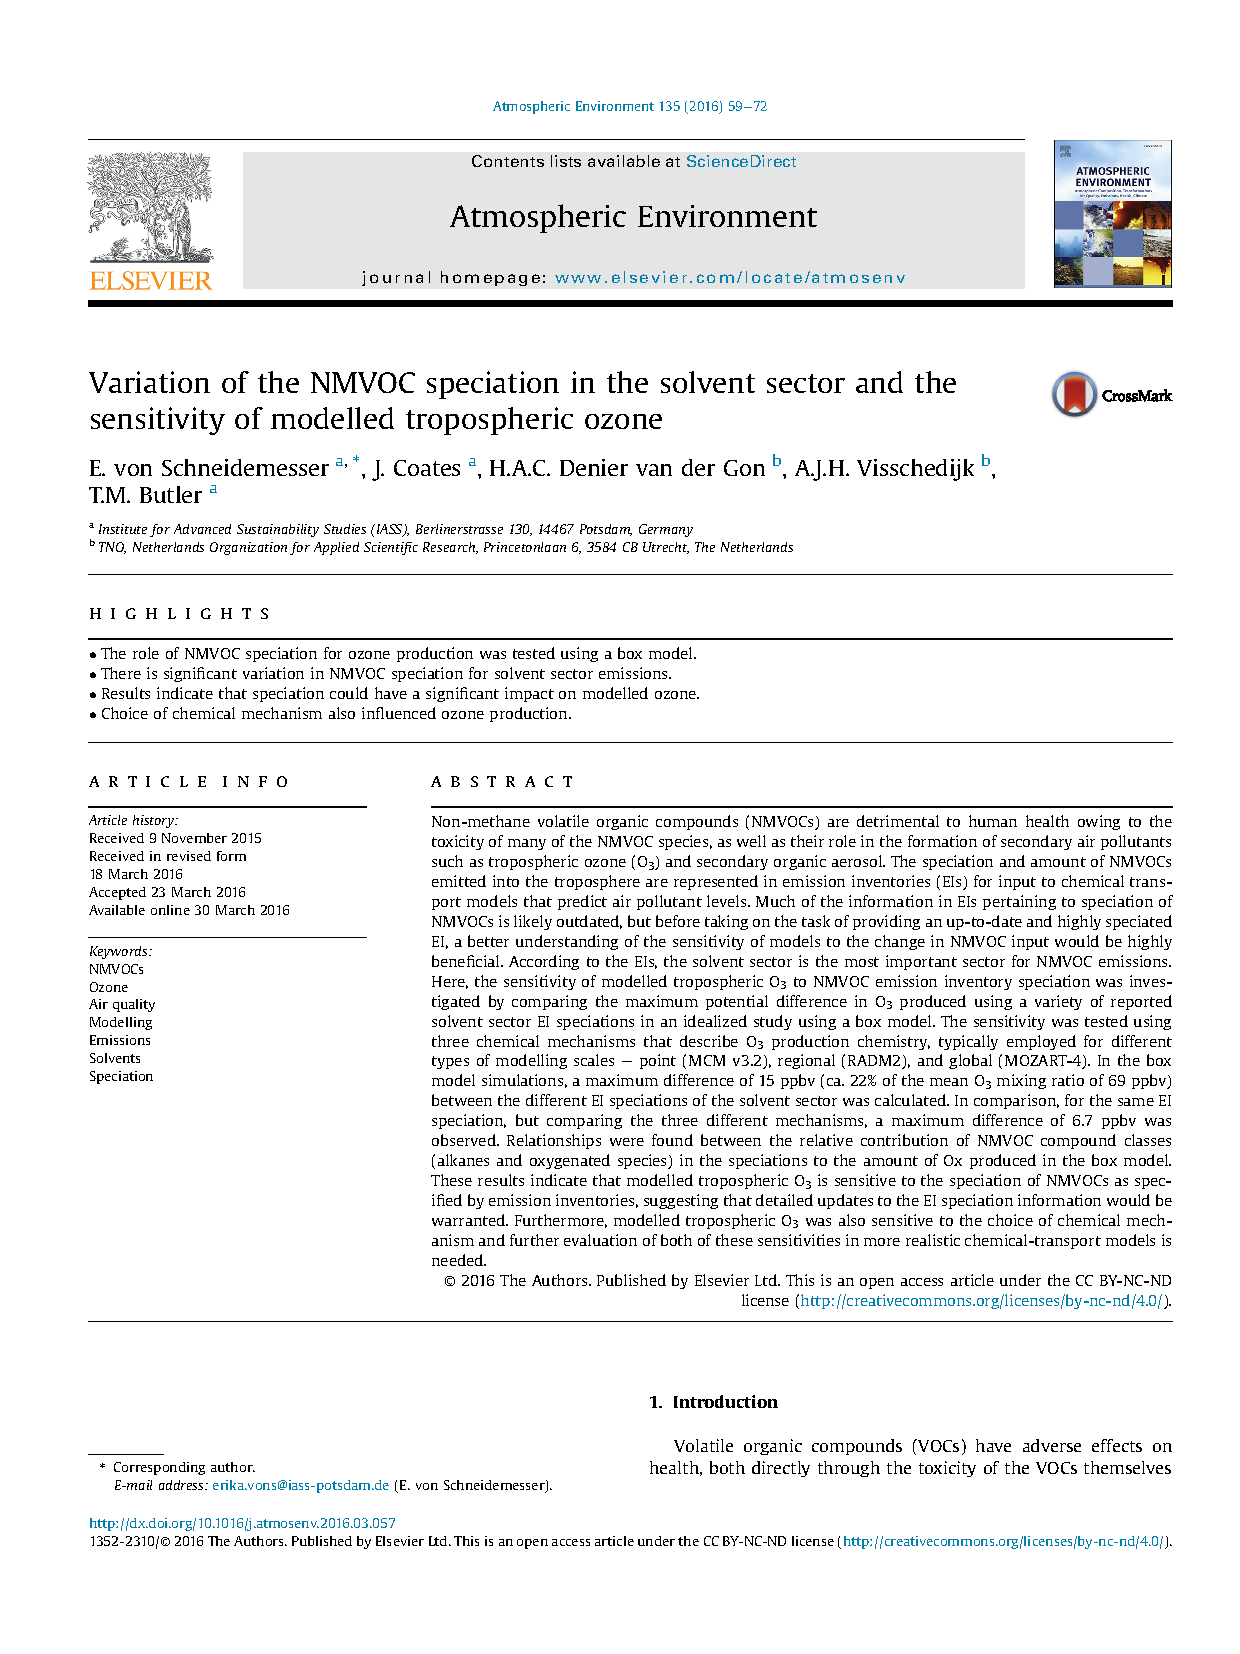
\includepdf[pages=-]{img/paper2.pdf}
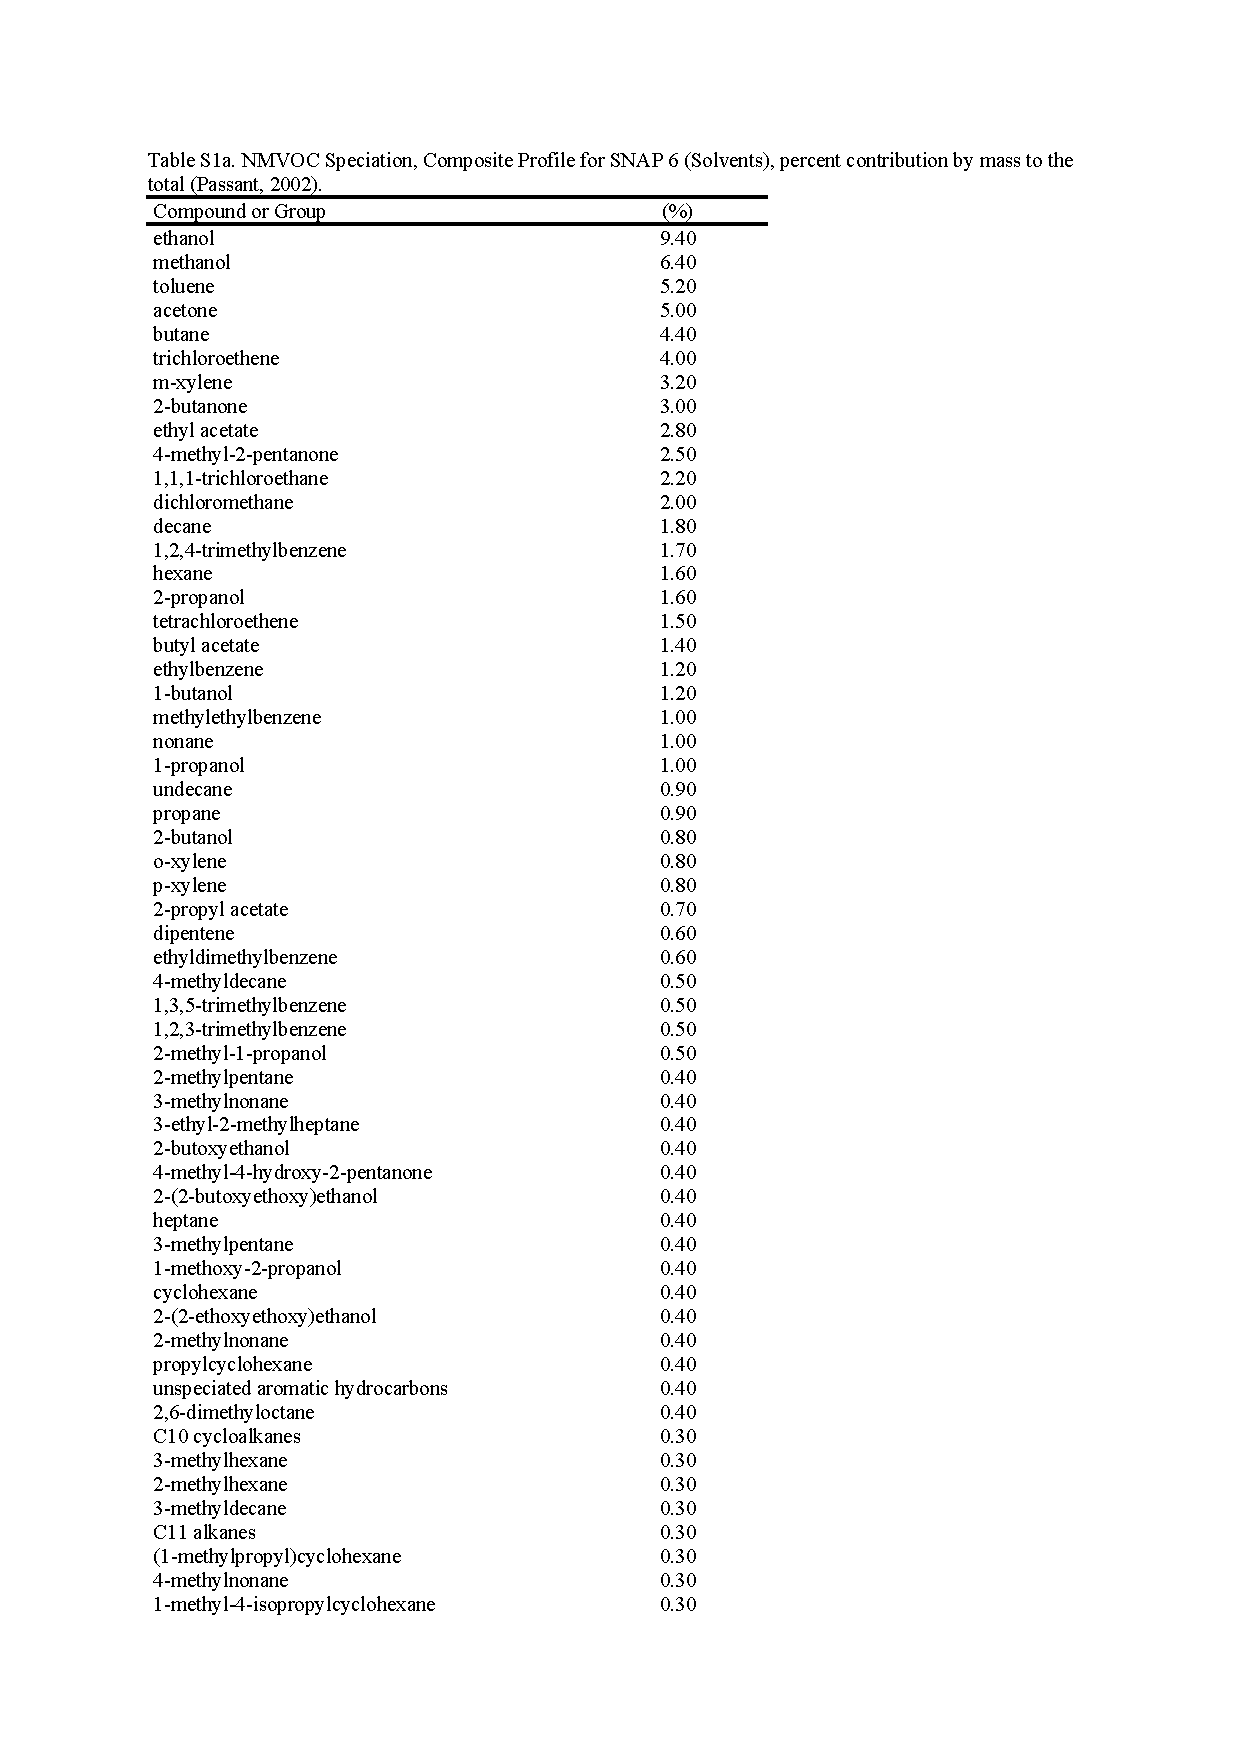
\includepdf[pages=-]{img/paper2-supplement.pdf}

\chapter{Paper III: The Influence of Temperature on Ozone Production under varying \ce{NO_x} Conditions -- a modelling study} \label{c:paper_3}
\clearpage{\pagestyle{empty}\cleardoublepage}
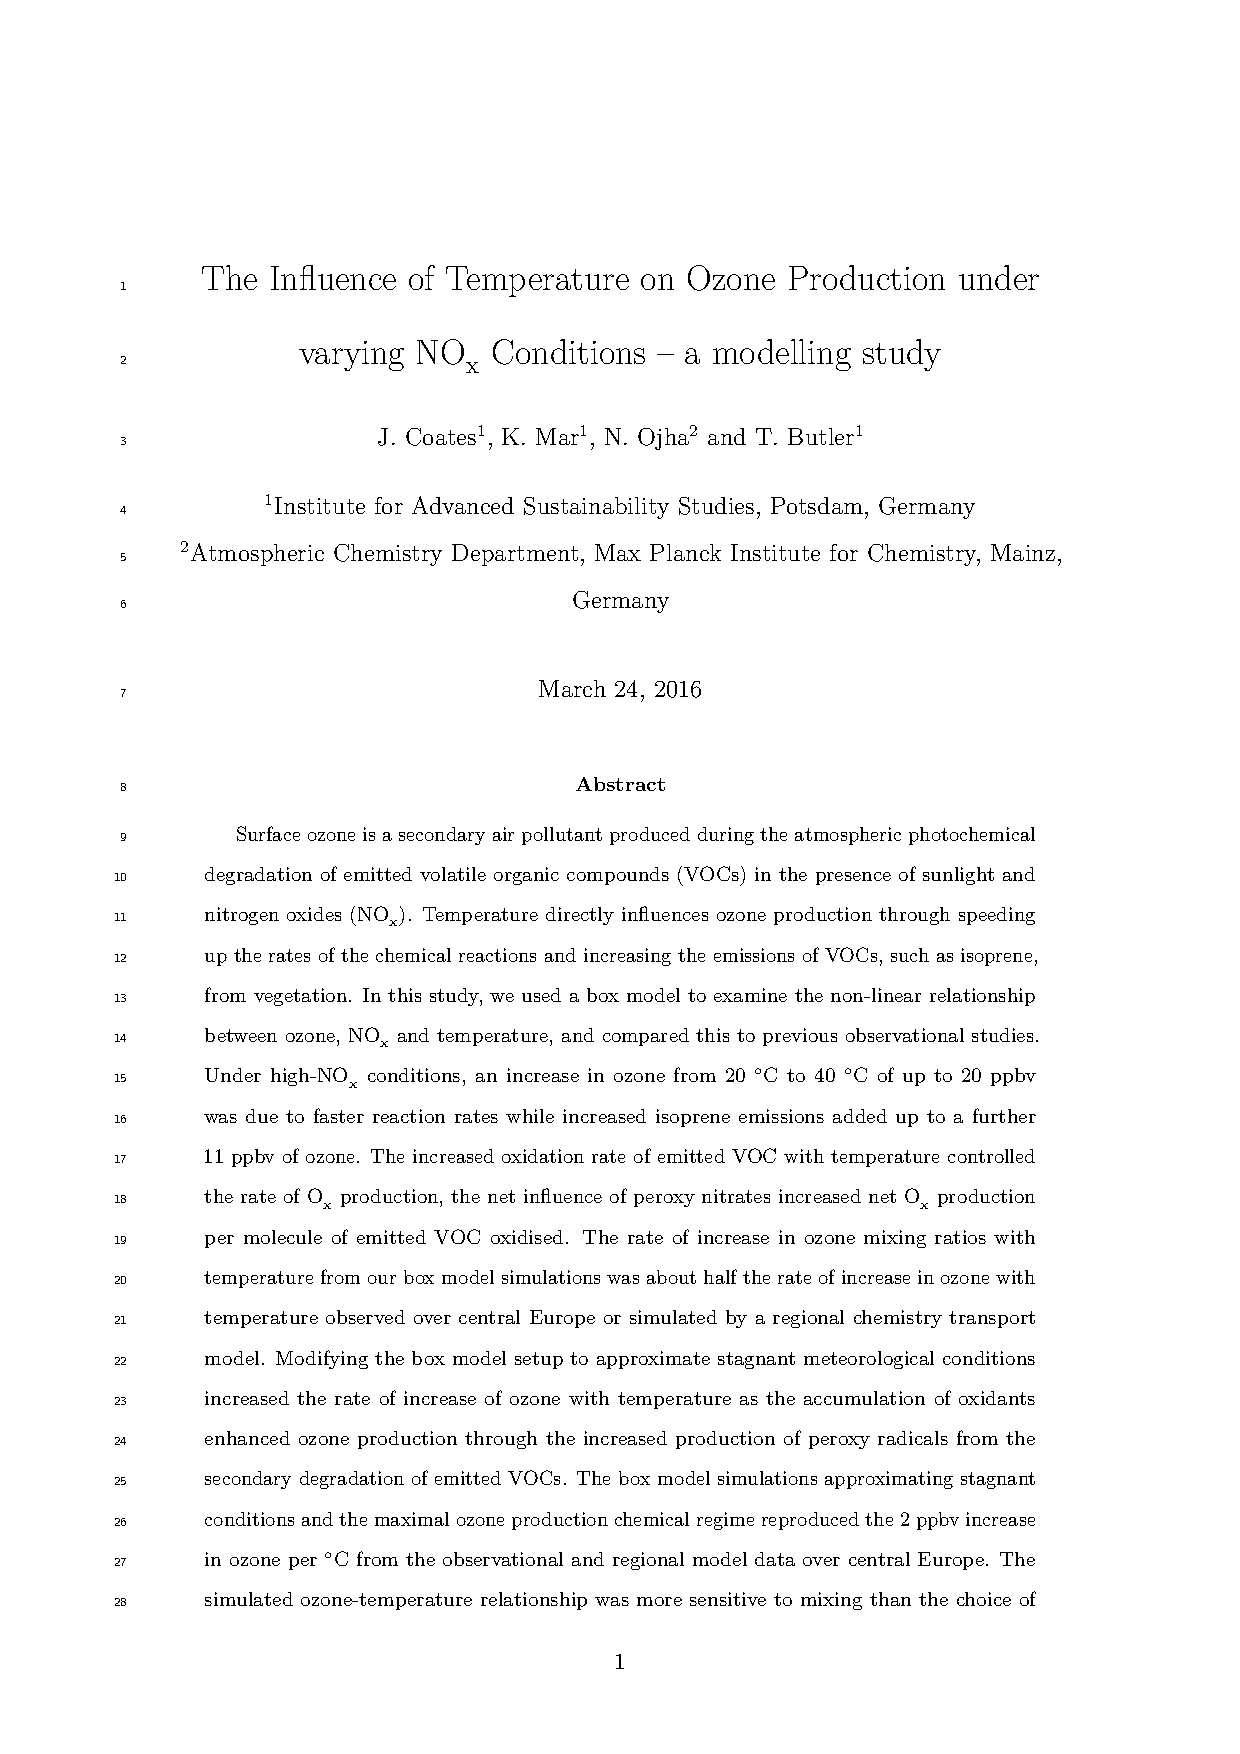
\includepdf[pages=-]{img/paper3.pdf}
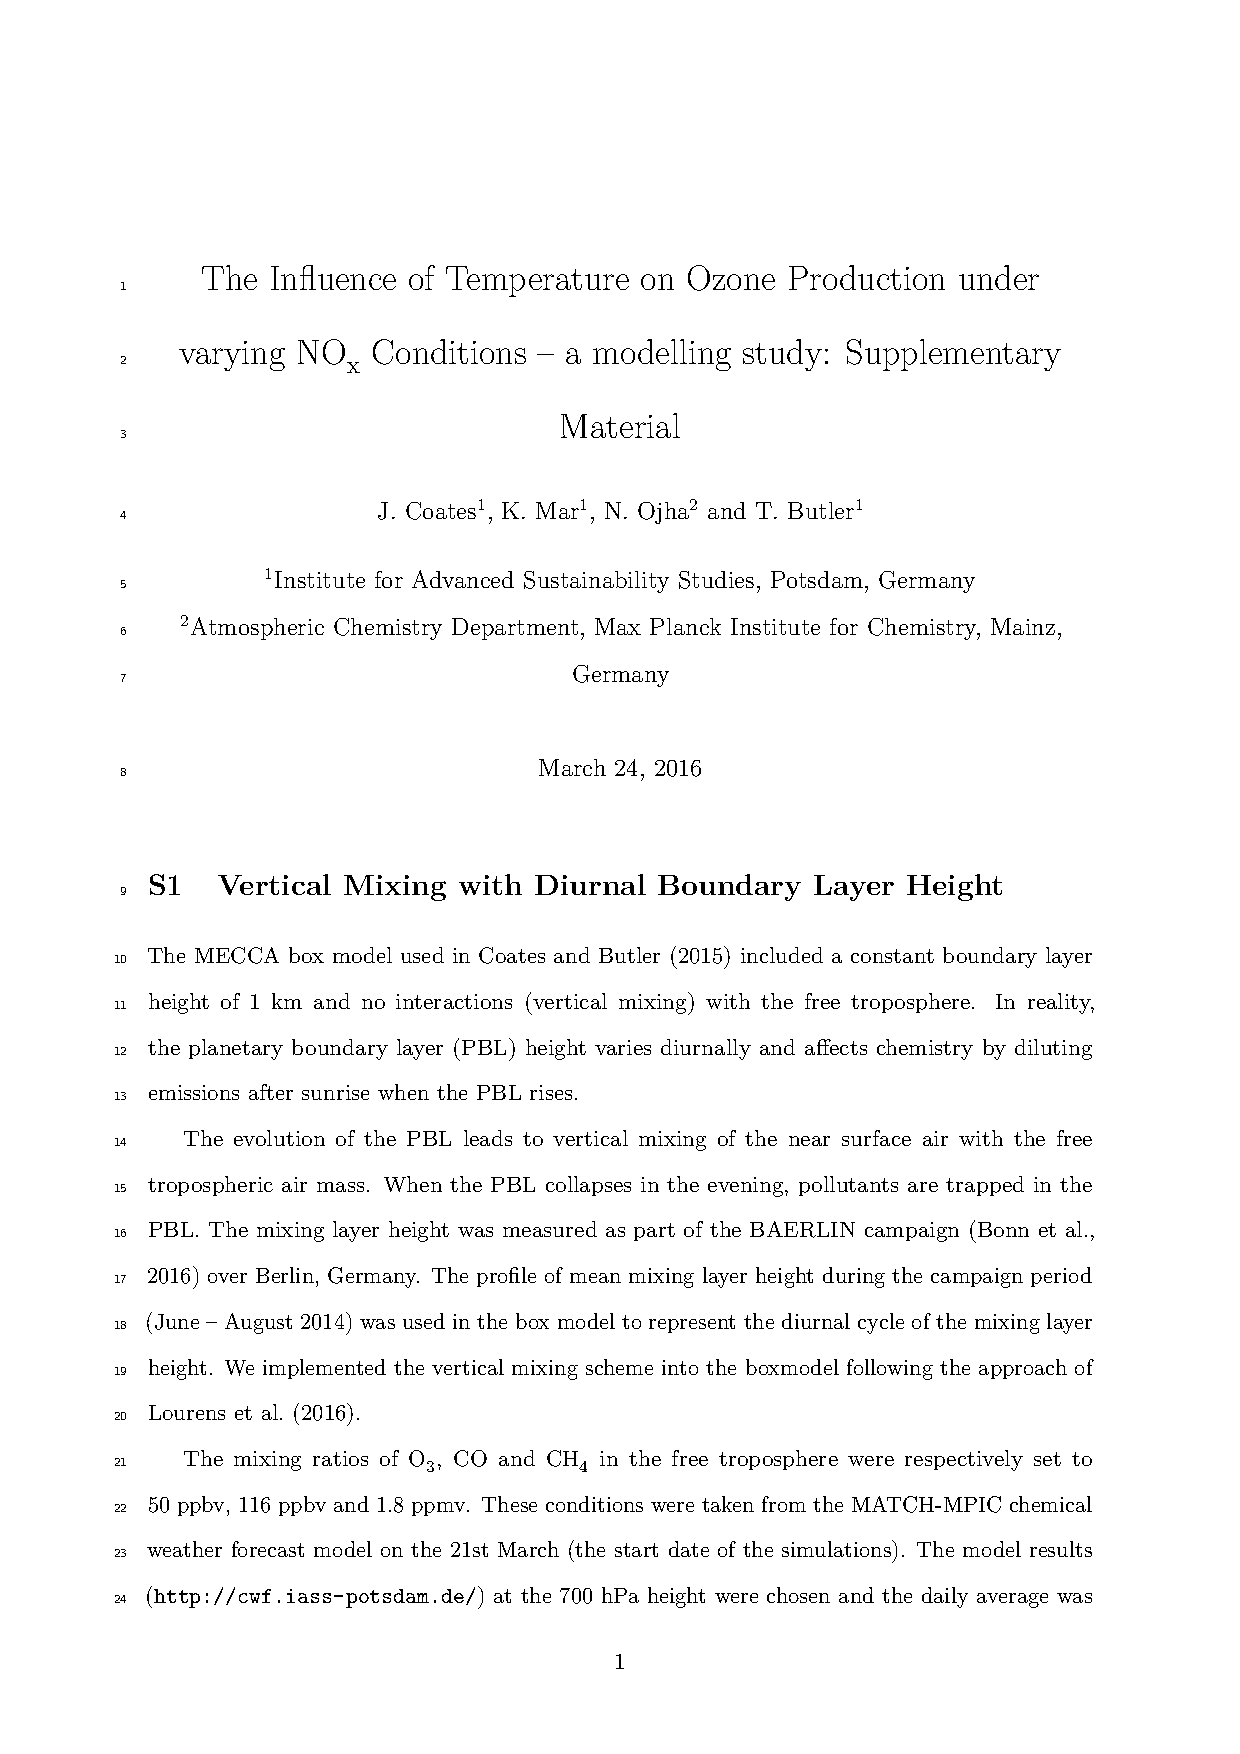
\includepdf[pages=-]{img/paper3-supplement.pdf}

\fancyhead[LO,RE]{Chapter \thechapter}
\chapter{Publication List}
\section{Scientific Articles}
\setlength{\parindent}{0pt}{
    \bibentry{Coates:2015}.

    \bibentry{vonSchneidemesser:2016}.

    \bibentry{Coates:2016}.
}

\section{Presentations}
\setlength{\parindent}{0pt}{
    J. Coates and T. M. Butler, Comparing chemical mechanisms using Tagged Ozone Production Potentials. 2013 American Geophysical Union Fall Meeting, 10th December 2013.

    J. Coates and T. M. Butler, Comparing how chemical mechanisms treat VOC degradation and impact on ozone production. 2014 PhD Conference on Earth System Science, 13th March 2014.

    \newpage
    J. Coates and T. M. Butler, The influence of atmospheric conditions on the production of ozone during VOC oxidation. 2015 American Geophysical Union Fall Meeting, 15th December 2015.
}

\section{Posters}
\setlength{\parindent}{0pt}{
    J. Coates and T. M. Butler, Comparing how chemical mechanisms treat VOC degradation and impact on ozone production. 2014 PhD Conference on Earth System Science, 13th March 2014.

    J. Coates and T. Butler, Understanding ozone pollution: a comparison of chemical mechanisms. 2014 Our Climate Our Future Conference, 7th October 2014.
}

\clearpage{\pagestyle{empty}\cleardoublepage}

\addcontentsline{toc}{chapter}{Appendix}
\chapter*{Appendix}
\noindent
Contribution to Paper I:

The experimental setup was designed by Tim Butler, the tagging of all chemical mechanisms and all model simulations performed by myself at the IASS.
All analysis and graphical plotting of the model output data was performed by myself.
The paper was written by myself assisted by Tim Butler.

\noindent
Contribution to Paper II:

The experimental setup was formulated by Erika von Schneidemesser, Tim Butler and myself.
Translating the NMVOC emissions into chemical mechanism species was performed by myself aided by Erika von Schneidemesser and colleagues at TNO.
All model simulations and analysis of model data was performed by myself at the IASS.
I prepared an initial draft of the paper which was further updated by Erika von Schneidemesser and the other co-authors.

\noindent
Contribution to Paper III:

The experimental setup was designed by Tim Butler any myself.
I updated the box model setup to include vertical mixing and a diurnal PBL height, and performed all model simulations at the IASS.
Observational data was provided by Noelia Otero Felipe and WRF-Chem model output by Kathleen A. Mar and Narendra Ojha.
Analysis and graphical plotting of the box model output data was performed by myself.
The paper was written by myself aided by the co-authors.


\end{document}
